% concatenated from arxiv-submission.tex, Bookkeeping/Graphics/preable.tex
\documentclass{article}


\usepackage{amsmath,amssymb,amsfonts,amsthm}
\usepackage[numbers]{natbib}
\usepackage[colorlinks,citecolor=blue,urlcolor=blue]{hyperref}
\usepackage[utf8]{inputenc}
\usepackage[T1]{fontenc}
\usepackage{microtype}
\usepackage{fullpage}
\usepackage{mathrsfs}
\usepackage{dsfont}
\usepackage{todonotes}
\usepackage{subcaption}

\newtheorem{definition}{Definition}[section]
\newtheorem{lemma}{Lemma}[section]
\newtheorem{theorem}{Theorem}[section]
\newtheorem{proposition}{Proposition}[section]
\newtheorem{corollary}{Corollary}[section]
\newtheorem{remark}{Remark}[section]
\newtheorem{question}{Question}[section]
\newtheorem{conjecture}{Conjecture}[section]

\newcommand{\eqdef }{\ensuremath{\stackrel{\mbox{\upshape\tiny def.}}{=}}}
\newcommand{\ReLU}{\operatorname{ReLU}}
\newcommand{\ICG}{\mathrm{IC_G}}
\newcommand{\ICR}{\mathrm{IC_R}}
\newcommand{\AG}{\mathrm{A_G}}
\newcommand{\AR}{\mathrm{A_R}}

\usepackage{xcolor}
\definecolor{almostblack}{RGB}{20,20,20}
\definecolor{charcoalblack}{RGB}{28,28,28}

% cool question box
\usepackage[most]{tcolorbox}

\newtcolorbox{questionbox}{
  enhanced,
  hbox,
  colback=gray!6,
  colframe=gray!50,
  boxrule=0.4pt,
  arc=1.5mm,
  left=3mm,
  right=3mm,
  top=1.2mm,
  bottom=1.2mm,
  before=\begin{center},
  after=\end{center}
}
\usepackage{tikz}
\usetikzlibrary{arrows.meta}
\usepackage{xcolor,amsmath}

\definecolor{nearblack}{RGB}{20,20,20}
\definecolor{lightgraytext}{RGB}{175,175,175}
\definecolor{gridgray}{RGB}{190,190,190}

\definecolor{myblue}{RGB}{35,85,205}
\definecolor{myred}{RGB}{215,60,50}

% colours chosen to go roughly from green (small) to red (large),
% based on the height of each hat
\definecolor{hatone}{RGB}{170,190,70}
\definecolor{hattwo}{RGB}{215,70,55}
\definecolor{hatthree}{RGB}{60,160,60}
\definecolor{hatfour}{RGB}{235,155,45}
\definecolor{hatfive}{RGB}{200,55,50}
\definecolor{hatsix}{RGB}{220,120,50}


\definecolor{levelone}{RGB}{85,150,60}
\definecolor{leveltwo}{RGB}{245,150,30}
\definecolor{levelthree}{RGB}{235,95,35}
\definecolor{levelfour}{RGB}{210,35,35}
\newcommand{\pp}[1]{\textcolor{magenta}{#1}}
% \newcommand{\eqdef }{\mathrel{\stackrel{\scriptscriptstyle\mathrm{def}}{=}}}


\title{Adaptivity Under Realizability Constraints:\\
Comparing In-Context and Agentic Learning}

\author{Anastasis Kratsios\thanks{McMaster University and the Vector Institute, Main St., Hamilton, L8S 4L8, Ontario, Canada, email: \texttt{kratsioa@mcmaster.ca}} \footnotemark[4] \and A. Martina Neuman \thanks{University of Vienna, Faculty of Mathematics, Kolingasse 14-16,
    1090 Wien, Austria, 
    e-mail: \texttt{anh.martina.neuman@univie.ac.at}
  } \footnotemark[4] \and Philipp Petersen \thanks{
    University of Vienna,
    Faculty of Mathematics and Research Network Data Science @ Uni Vienna, Kolingasse 14-16,
    1090 Vienna, Austria, 
    e-mail: \texttt{philipp.petersen@univie.ac.at}
  } \thanks{All authors contributed equally}}
\date{May 2026}

\begin{document}

\maketitle

\begin{abstract}
We compare in-context learning with fixed queries and 
agentic learning with adaptive queries for uniform
approximation of task families. 
We consider two settings: 
an unrestricted regime,  
where querying and approximation are  
arbitrary functions, and a realizable regime, 
where we require these operations to be implemented by ReLU neural networks. 
In both settings, adaptivity never hinders approximation performance. 
However, this advantage can change when one passes from the unrestricted regime to the realizable regime.
We identify four distinct approximation scenarios, each witnessed by an explicit task family: (a) no advantage of adaptivity; (b) an advantage in the unrestricted regime that persists under ReLU realizability; (c) an advantage that arises only under realizability; and (d) an advantage that disappears under realizability.
This demonstrates that representational constraints interact profoundly with the effect of adaptivity.
\end{abstract}

\section{Introduction}

Modern learning systems exhibit %have a 
well-documented few-shot~\cite{brown2020,li2025transformers} and \emph{multi-task}~\cite{Caruana1997Multitask,ArgyriouEvgeniouPontil2008ConvexMTL,MishraEtAl2022NaturalInstructions,WangEtAl2022SuperNaturalInstructions} learning capabilities. 
These recent advances are largely attributed to their ability to access task information through prompts \cite{brown2020}, retrieved examples \cite{lewis2020rag}, memory \cite{park2023generative}, or sequential interaction with an environment \cite{yao2023react}. %; \cite{brown2020,lewis2020rag,park2023generative,yao2023react}. 
Fixed prompts are an instance of \emph{in-context learning} (ICL), while sequential interaction leads to \emph{agentic learning}. 
For a mathematically tractable treatment, we adopt a viewpoint in which sequential interaction consists of adaptive query selection based on past observations, whereas prompts are fixed queries specified a priori.
The central question of this article is simple: \emph{when does sequential interaction actually help, and how does that answer change once realizability constraints are imposed?}
%Someone always wants to put this question into different formats. I think the intro should not be overleaded with different types of displays and we already have the regimes, the table, the bullet point list and an equation. That is why I always change this back :D.

To this end, we compare four regimes, defined formally in Section~\ref{sec:setup}:
\begin{align*}
&\ICG \;\text{(general in-context)},&
\qquad
&\ICR \;\text{(ReLU in-context)},\\
&\AG \,\,\;\text{(general agentic)},&
\qquad
&\AR \,\,\;\text{(ReLU agentic)}.
\end{align*}
%For our purposes, an in-context learner is a function that is allowed access to fixed, but arbitrary samples. On the other hand, an agentic learner (or ``agent'') is an approximation method that can choose its samples adaptively. 
For our purposes, an in-context learner is a function that can access a fixed (but arbitrary) collection of samples, whereas an agentic learner (or ``agent'') selects its samples adaptively based on past observations.
Both learners %methods 
are required to approximate an entire given class of functions. 
Along a second axis, we distinguish between %the distinction 
\emph{general} approximators and \emph{ReLU-realizable} (or simply \emph{realizable}) approximators. %is as follows: 
%Here ``general'' means that no representability restriction is imposed on the learner, whereas the realizability regimes require the querying mechanism and the final predictor %overall functions be implemented by bounded-size ReLU networks. 
A general approximator is subject to no representational restriction; a realizable one requires both the querying mechanism and the final predictor to be implemented by bounded-size ReLU networks.
Formal definitions are provided in Section \ref{sec:setup}. 

To understand the relationship in terms of approximation power between the introduced regimes, %methods above, 
%we always compare approximation uniformly for a given \emph{full function class} and assume methods that are compared to have access to the same number of samples and the same computational budget for the involved ReLU networks. 
we consider uniform approximation over a given \emph{full function class} and assume equal sample budgets and, where applicable, equal computational budgets for the underlying ReLU networks.
An immediate observation is the monotonicity
\begin{align}
\label{eq:adaptivityCannotHurtAnyone}
\ICG\leq \AG,
\quad\text{ and }\quad
\ICR\leq \AR,
\end{align}
which holds for \emph{all} function classes. 
Here ``$\leq$'' means that the method on the right does not incur a larger worst-case uniform approximation error than the one on the left. %uniformly over the said function class. 
%The reason for \eqref{eq:adaptivityCannotHurtAnyone} is that the option to adaptively choose samples can never hurt, because an agent can always ignore it and imitate a fixed sampling rule. 
The inequality \eqref{eq:adaptivityCannotHurtAnyone} follows from the fact that adaptive sampling can always be ignored, so an agent can imitate any fixed sampling rule.
We formalize this fundamental fact in Proposition~\ref{prop:monotonicity}.
In the sequel, we will also use the symbol ``$=$'' to denote that both methods yield the same worst-case error (over an underlying function class) and $<$ to denote that the method on the right yields a strictly smaller worst-case error than the one on the left. 
We give a formal definition of these relations in Definition \ref{def:formalDefRelations}.

Apart from the case $\ICG=\AG$ and $\ICR=\AR$---which already occurs for every singleton task
family---%in which adaptivity helps at neither level, only three nontrivial configurations remain:
in which adaptivity yields no improvement, only three nontrivial configurations remain:

\begin{center}
\begin{tabular}{lcc}
\hline
\textbf{Phenomenon} & \textbf{General} & \textbf{ReLU-realizable} \\
\hline
adaptivity advantage survives realizability & $\ICG<\AG$ & $\ICR<\AR$ \\
realizability generates adaptivity advantage & $\ICG=\AG$ & $\ICR<\AR$ \\
adaptivity advantage removed by realizability & $\ICG<\AG$ & $\ICR=\AR$ \\
\hline
\end{tabular}
\end{center}

%The point of this article is to isolate all three nontrivial patterns. 
In the main results, we isolate all three of these nontrivial configurations.
Concretely,
Theorems~\ref{thm:path}, \ref{thm:value}, and \ref{thm:address} identify function classes realizing each of these patterns, which may be distinguished as follows: %of the patterns. 
%Consequently, these are distinct as:
\begin{itemize}
    \item \emph{adaptivity reveals more information}: on \emph{cubical-path} tasks, adaptive querying
    reveals strictly more task information than every fixed context, and this advantage survives the
    ReLU-realizability restriction; see Section~\ref{s:Main__ss:pathada_realizability};
    \item \emph{adaptivity bypasses internal computation}: on the \emph{pointed-value} family,
    unrestricted in-context and unrestricted agentic learning are equally powerful, but a ReLU-realizable
    agentic learner can bypass a hard internal computation that a ReLU-realizable in-context learner needs to perform; %by reading the needed quantity from one extra adaptive query; 
    see Section~\ref{s:Main__ss:realizabilityonly};
    \item %\emph{adaptivity itself requires hard computation}: 
    \emph{adaptivity is limited by hard computation}:
    on the \emph{address-spike} family,
    unrestricted adaptivity provides strict approximation gains, %again helps, 
    but now the informative adaptive query location is computationally hard to determine; %itself hard to compute, 
    consequently, %a natural 
    bounded-size %one-step 
    ReLU agents %ic protocol 
    lose these gains; %this advantage; 
    see
    Section~\ref{s:Main__ss:killed-by-realizability}.
\end{itemize}

This yields the promised conceptual classification: \emph{once realizability is taken into account,
adaptivity advantages can survive, appear, or disappear}. 






\section{Related work}



\paragraph{In-context learning.}
Our notion of in-context learning is motivated by the modern few-shot prompting paradigm for large
language models, where task information is supplied through examples or instructions at inference time rather than through parameter updates \cite{brown2020}. 
On the theoretical side, recent work studies what 
function classes can learn from such fixed in-context examples for \emph{structured families}, typically exploiting shared low complexity across tasks, particularly in transformer architectures \cite{akyurek2023what, garg2022}. 
While related in spirit, we use structured families from a different perspective: to highlight the role of adaptive information acquisition and to characterize how realizability alters its advantage.
In our formulation, this corresponds to an \emph{agent}, possibly realized by a ReLU network, that adaptively selects which inputs to query and updates its predictor based on the observed responses.

We distinguish our approximation-theoretic lens from the statistical lens that typically dominates the ICL literature. In particular, our focus differs from work on scaling laws~\cite{bordelon2025theory}, simplified attention mechanisms that learn linear tasks in context~\cite{wu2023many,zhang2024trained}, the low-frequency inductive bias of trained transformers~\cite{yang2025provable}, and algorithmic perspectives in which ICL implements an implicit learning algorithm within the forward pass~\cite{vonoswald2023what} or, more broadly, a meta-learning procedure that maps in-context examples directly to a predictor or its parameters~\cite{chen2022transformers}.
These approaches operate on a given prompt of in-context examples and therefore do not address adaptive information acquisition or how it interacts with architectural constraints and realizability.


\paragraph{Adaptive sampling, active learning, and information-based complexity.}
The adaptive %side of our note 
component of our learning model is closely related to classical \emph{query learning} and \emph{active learning}, where a learner chooses which information to reveal %next on the basis of past observations. 
based on past observations, viewed as sequentially acquired examples.
Membership- and equivalence-query models already highlight the power of adaptive access to an unknown target through sharp bounds on \emph{query complexity}, see e.g. \cite{angluin1987}, while the active learning literature studies how %the benefit of 
sequential sample selection reduces label complexity for generalization \cite{cohn1994,dasgupta2011}. 
Adaptive sampling frameworks similarly study how measurements can be chosen on-the-fly to improve estimation accuracy for structured signal classes \cite{castro2009active, sung1994active}.
More broadly, %these perspectives also close in spirit to 
our setting is most closely aligned with the framework of \emph{information-based complexity}, which studies the
intrinsic difficulty of approximation %and numerical problems 
under partial information and restricted
access to the target object. %(e.g.\ using a limited budgets of bits to encode it~\cite{kolmogorov1959varepsilon}, or often linear~\cite{pinkus2012n,krieg2021function,adcock2025optimal} but sometimes non-linear $1$-Lipschitz~\cite{cohen2022optimal,petrova2023lipschitz} measurements/queries). 
This framework was formalized in the 1980s in \cite{packel1987ibc, traub1988ibc} and further developed in \cite{novak2008tractability}, where approximation under partial information is modeled via prescribed \emph{information operators} (typically a collection of linear or nonlinear functionals), and complexity is measured by the minimal achievable error.
Modern developments consider a range of information models, including limited bit encodings \cite{kolmogorov1959varepsilon}, linear measurements \cite{pinkus2012n, krieg2021function, adcock2025optimal}, and nonlinear (e.g., $1$-Lipschitz) queries \cite{cohen2022optimal}.



\paragraph{Multi-tasking and connections to operator learning.}
The shift from the classical universal approximation perspective, where only a single task is approximated, to the approximation of task families remains only partially explored in ICL. 
%This places our work within the broader adjacent field of approximation theory for \emph{operator learning}, where a large family of what can be interpreted as ``multi-task'' approximation guarantees is available~\cite{ChenChen1995Operators,LiEtAl2021FNO,KovachkiEtAl2023NeuralOperator,KovachkiLanthalerMishra2021FNOTheory,LanthalerMishraKarniadakis2022DeepONetError,kratsios2025generative,furuya2025one,lanthaler2025nonlocality,galimberti2026designing}. 
This places our work within the broader context of approximation theory for \emph{operator learning}, where many results admit an interpretation as ``multi-task'' approximation guarantees~\cite{furuya2025one, KovachkiEtAl2023NeuralOperator, KovachkiLanthalerMishra2021FNOTheory, LanthalerMishraKarniadakis2022DeepONetError, kratsios2025generative, LiEtAl2021FNO}.
Those results, together with the first ICL approximation result of~\cite{li2025transformers}, suggest that multi-task learning may be subject to significant %\emph{exponentially-large} 
information-theoretic bottlenecks, %/\emph{lower-bounds}, 
similar to those encountered in neural operator approaches to simultaneously solving families of scientific computing problems~\cite{lanthaler2026parametric}. 
%The objective of this paper, however, is \emph{not} to characterize the \emph{worst-case} scaling of arbitrary multi-task approximation frameworks; rather, it is to identify settings where context and agency unlock favorable, or at least improved, approximation rates, echoing the work of~\cite{Barron1991ComplexityRegularization,Barron1993UniversalApproximation,mhaskar2017and}, which uncovered regimes where efficient approximation by MLPs is possible in the context-free early deep-learning setting.
The objective of our paper, however, is not to characterize worst-case scaling laws of arbitrary multi-task approximation frameworks, but to isolate how adaptive information acquisition interacts with realizability constraints.
%In particular, we identify regimes in which adaptivity provides a strict advantage, regimes in which this advantage arises only under realizability constraints, and regimes in which it disappears.
This perspective extends classical results on non-adaptive approximation by MLPs~\cite{Barron1993UniversalApproximation,mhaskar2017and}, suggesting that beyond function class complexity, the structure of information acquisition---such as adaptivity---also plays a central role.

\paragraph{Approximation-theoretic setting.}
%Finally, our realizability constraints place the discussion in the approximation-theoretic setting of ReLU networks, where both upper and lower bounds are well understood for broad function classes, see \cite{petersen2024mathematical} for an overview. The contribution of this note is to compare these two axes: adaptivity and ReLU-realizability, within one uniform approximation framework. This allows us to study how adaptivity interacts with representational constraints, which is central to the phenomena identified in this work.
The contribution of this note is to compare two axes---adaptivity and ReLU realizability---within a uniform approximation framework. This allows us to study how adaptivity interacts with representational constraints, which is central to the phenomena studied here. Imposing realizability constraints, in turn, places the discussion in the well-studied setting of ReLU networks, where both upper and lower bounds are available; see~\cite{petersen2024mathematical} for an overview.

We note that many of our results can be extended to multi-head transformers, and are therefore not MLP-specific, via our MLP-to-transformer conversion; see Proposition~\ref{prop:transformerification__SparseVersion} and the discussion in Remark \ref{rem:transformers}. 
This mirrors~\cite[Proposition 11]{kratsios2025context} for our standard notion of attention, and is consistent with similar conversion results for CNNs~\cite{petersen2020equivalence}, spiking neural networks~\cite{dold2026equivalence, neuman2025stable}, and transformers~\cite{hu2026transformerapproximationsrelus}. 
%%


\section{Setup}\label{sec:setup}


Throughout, $\mathcal X\subseteq \mathbb R^d$ is compact, $\mathcal{T}\subseteq\{f:\mathcal X\to
\mathbb R\}$ is a family of tasks, and approximation is measured in the uniform norm
$\|\cdot\|_{L^\infty(\mathcal X)}$.  We consider $\operatorname{ReLU}$-MLPs and transformers with multi-head attention and $\operatorname{ReLU}$ activation functions; see Appendix~\ref{s:models} for standard definitions. 

Let $f\in\mathcal T$. For $n\in\mathbb N$ and query points $x_1,\dots,x_n\in\mathcal X$, we write
\[
C_n(f;x_1,\dots,x_n)\eqdef  ((x_i,f(x_i)))_{i=1}^n
\]
for the ordered \emph{context} gathered from the task $f$. 
Since we study the limits of %expressivity
adaptivity under realizability constraints, we do not include noise in the measurements $f(x_i)$, so as to isolate the core phenomena.
This is in part in line with standard approximation theory~\cite{yarotsky2017,petersen2018optimal,kratsios2022universal}.
%This is in line with standard approximation theory~\cite{hornik1990universal,yarotsky2017,petersen2018optimal,kratsios2022universal}. 
%We also note that even the context-free uniform approximation theory for MLPs is not developed in the presence of noise; to the best of our knowledge, only the following result is currently available~\cite{kratsios2025beyond} for uniform error quantification.
Uniform (worst-case) approximation results for neural networks are typically formulated in this noise-free setting, while quantitative results incorporating noise remain comparatively limited; see, e.g., \cite{kratsios2025beyond}.



\begin{definition}[In-context learners]
Fix a sample budget $N\in\mathbb N$. A \emph{general in-context learner} $\Psi_{\rm IC}$ consists of fixed query points $x_1,\dots,x_N\in\mathcal X$ and a predictor
\[
 \widehat{F}_{\Psi_{\rm IC}}:(\mathcal X\times\mathbb R)^N\times\mathcal X\to\mathbb R,
\]
which, for a task $f\in\mathcal T$, outputs the function
\[
x\mapsto \Psi_{\rm IC}(f)(x) \eqdef 
\widehat{F}_{\Psi_{\rm IC}}
(C_N(f;x_1,\dots,x_N),x).
\]
We say that $\Psi_{\rm IC}$ is a \emph{ReLU-realizable in-context learner} (or \emph{realizable}) if it is represented by a bounded-size ReLU network. 
%The size of the ReLU in-context learner is defined as the size of $\Psi_{\rm IC}$.
The size (i.e.\ number of non-zero parameters or network weights) of the ReLU network involved is defined as the size of $\Psi_{\rm IC}$.
\end{definition}



\begin{definition}[Agentic learners]
Fix a query budget $N\in\mathbb N$. A \emph{general agentic learner} $\Psi_{\rm A}$ consists of an initial
query point $x_1\in\mathcal X$, adaptive query maps
\begin{equation} \label{querymaps}
    q_n:(\mathcal X\times\mathbb R)^{n-1}\to\mathcal X,
    \qquad n=2,\dots,N,
\end{equation}
and a final predictor
\[
\widehat{F}_{\Psi_{\rm A}}:(\mathcal X\times\mathbb R)^N\times\mathcal X\to\mathbb R.
\]
For a task $f\in\mathcal T$, the resulting query sequence is defined recursively by
\[
x_1(f)\eqdef  x_1,
\qquad
x_n(f)\eqdef  q_n\bigl(C_{n-1}(f;x_1(f),\dots,x_{n-1}(f))\bigr),
\quad n=2,\dots,N,
\]
and the learner $\Psi_{\rm A}$ outputs the function
\begin{equation} \label{finpredictor}
    x\mapsto \Psi_{\rm A}(f)(x) \eqdef 
 \widehat{F}_{\Psi_{\rm A}}
 \bigl(C_N(f;x_1(f),\dots,x_N(f)),x\bigr).
\end{equation}
We say that $\Psi_{\rm A}$ is a \emph{ReLU-realizable agentic learner} (or \emph{realizable}) if the adaptive query maps and final predictor can all be
implemented by bounded-size ReLU networks. 
The size (i.e.\ number of non-zero parameters or network weights) of the largest of the involved ReLU networks is called the size of $\Psi_{\rm A}$.
%the ReLU-realizable agentic learner.
\end{definition}


\begin{remark}
We do \emph{not} distinguish notationally between general learners, in-context or agentic, and their realizable counterparts.
In particular, the symbols $\Psi_{\rm IC}$ and $\Psi_{\rm A}$ may denote either type.
\end{remark}


The complexity of our networks is quantified via resource budgets. We distinguish between a \emph{query budget} $N$, corresponding to the number of samples, and a \emph{weight budget} $m$, corresponding to the network size (for realization). 
In the realizable regimes $(\ICR, \AR)$, both budgets, i.e. $(N,m)$, are imposed. In contrast, for the general regimes $(\ICG, \AG)$ no restriction on the class of functions used is imposed, so a weight budget is not applicable. There, only the query budget $N$ is constrained. All comparisons are made under matching query budgets, and, when applicable, matching weight budgets.
%We now fix the relations between $\ICG, \AG, \ICR$, and $\AR$. 
We now define a comparison relation between the regimes $\ICG, \AG, \ICR$, and $\AR$. 
%The complexity of our networks are quantified in terms of a \emph{budget} on the network size; i.e.\ number of non-zero parameters.  It is in this way which we limit the \emph{information based complexity} of the learners in each regime.
% 



\begin{definition} \label{def:formalDefRelations}
%Fix a task family $\mathcal{T}$ and a query budget $N\in\mathbb N$, and, in the realizable regimes, an additional weight budget $m\in\mathbb N$. 
%For comparisons involving $\ICR$ or $\AR$, we additionally fix a {\color{red} weight} %ReLU-size 
%budget $m\in\mathbb N$. 
Fix a task family $\mathcal{T}$, a query budget $N\in\mathbb N$, and a weight budget $m\in\mathbb N$.
%For two regimes $\mathsf R_1,\mathsf R_2\in\{\ICG,\AG\}$ or $\mathsf R_1,\mathsf R_2\in\{\ICR, \AR\}$ or $\mathsf R_1,\mathsf R_2\in\{\ICG,\ICR\}$ or $\mathsf R_1,\mathsf R_2\in\{\AG, \AR\}$, we write
For $\{\mathsf R_1,\mathsf R_2\}\in \{\{\ICG,\AG\}, \{\ICR, \AR\}, \{\ICG,\ICR\}, \{\AG, \AR\}\}$, we write
\begin{equation*} 
    \mathsf R_1\leq \mathsf R_2
\end{equation*}
if for every learner $\Psi_1$ %$\mathcal L_2$ 
in regime $\mathsf R_1$ with the prescribed budgets there exists a learner $\Psi_2$ %$\mathcal L_1$ 
in regime $\mathsf R_2$ with the same prescribed budgets such that
\[
%\sup_{f\in\mathcal T}\|\mathcal L_2(f)-f\|_{L^{\infty}(\mathcal X)}
\sup_{f\in\mathcal T}\|\Psi_2(f)-f\|_{L^{\infty}(\mathcal X)}
\leq
%\sup_{f\in\mathcal T}\|\mathcal L_1(f)-f\|_{L^{\infty}(\mathcal X)}.
\sup_{f\in\mathcal T}\|\Psi_1(f)-f\|_{L^{\infty}(\mathcal X)}.
\]
Here, the budgets are understood as follows: 
\begin{itemize}
    \item in the general regimes $\{\ICG, \AG\}$ or in the cross-type regimes $\{\ICG,\ICR\}, \{\AG, \AR\}$, the query budget $N$ is imposed;
    \item in the realizable regimes $\{\ICR, \AR\}$, both query and weight budgets $(N,m)$ are imposed.
\end{itemize}
We write $\mathsf R_1=\mathsf R_2$ if both $\mathsf R_1\leq \mathsf R_2$ and $\mathsf R_2\leq \mathsf R_1$ hold, and we write $\mathsf R_1<\mathsf R_2$ if $\mathsf R_1\leq \mathsf R_2$ holds but $\mathsf R_2\leq \mathsf R_1$ does not.
\end{definition}

We emphasize that all relations are defined relative to a fixed task family and the relevant resource budgets; in particular, no comparison is meaningful without specifying them.

\begin{remark}
Technically the relation $\mathsf R_1\leq \mathsf R_2$ from Definition~\ref{def:formalDefRelations} can be extended to the case $\{\mathsf R_1,\mathsf R_2\}\in \{\{\ICG,\AR\}, \{\ICR, \AG\}\}$ under appropriate budget imposition. We do not directly consider these relations here, as they confound the effects of adaptivity and realizability and therefore do not isolate the contribution of adaptivity.
\end{remark}



\begin{remark} \label{rem:trivialRelation}
We note for future reference the obvious relations, %the obvious fact 
\begin{align*}
    \ICR \leq \ICG \quad \text{ and } \quad \AR \leq \AG,
\end{align*}
%which holds because all ReLU-realizable agentic learners are special cases of general agentic learners and the same holds for in-context learners. 
which follow from Definition~\ref{def:formalDefRelations}, since every realizable learner is a special case of a general learner.
\end{remark}

Our arguments often require a hard-to-approximate function. The following remark establishes the existence of one. 

\begin{remark}\label{rem:unattainableFunctions}
We shall repeatedly use the following standard fact: for every compact domain $\mathcal X\subseteq\mathbb R^d$, every weight budget $m$, and every compact interval $[a,b]$, there exists a continuous function with values in $[a,b]$ such that no ReLU network with at most $m$ weights can approximate it uniformly with error strictly smaller than $(b-a)/2$. To see this, assume toward a contradiction that every continuous function $f:\mathcal X\to[a,b]$ admits a ReLU network $\Phi_f$ with worst-case error smaller than $(b-a)/2$. 
Then for every $K \in \mathbb N$, every set of distinct points $(x_i)_{i=1}^K\subseteq \mathcal X$, and every label vector $(y_i)_{i=1}^K \in \{0,1\}^K$, there exists a continuous function $f:\mathcal X\to[0,1]$ such that $f(x_i)=y_i$ for all $i$. By assumption, the network $\Phi_{a+(b-a)f}$ then satisfies $\Phi_{a+(b-a)f}(x_i) > a+(b-a)/2$ if $y_i = 1$ and $\Phi_{a+(b-a)f}(x_i) < a+(b-a)/2$ if $y_i = 0$. Hence the class of ReLU networks with at most $m$ weights, composed with thresholding at $a+(b-a)/2$, shatters every finite set of distinct points in $\mathcal X$. This implies infinite VC dimension, contradicting \cite[Theorem 8.4]{AnthonyBartlett1999}. 
\end{remark}

In the sequel, we also occasionally use the following result: the existence of an $\varepsilon$-uniform $\operatorname{ReLU}$-MLP approximator $\operatorname{Mult}_{\varepsilon}$ of the binary multiplication function on $[0,1]^2$ %by a $\operatorname{ReLU}$-MLP, which we denote by $\operatorname{Mult}_{\varepsilon}$ 
with $\mathcal{O}(\log(1/\varepsilon))$ weights. The formal result is stated in Lemma~\ref{lem:approx-mult} and is due to~\cite{yarotsky2017}.

We close this section with two remarks on the limitations of this setup.

\begin{remark}
We focus on ReLU feed-forward neural networks because they provide a standard and well-understood
baseline in approximation theory. Most of the qualitative arguments of this paper extend to other
activation functions, provided three ingredients remain available:
\begin{itemize}
    \item One should exclude pathological activations for which fixed finite architectures already
    become universal approximators; see \cite{maiorov1999lower}.
    \item The activation should allow the construction of compactly supported bump functions as used in our separation examples. Higher-order ReLU
    activations are natural examples; for a general framework under fairly broad assumptions %, for a more refined discussion 
    see \cite{guhring2021encodable}.
    \item For the constructions in Section~\ref{s:Main__ss:realizabilityonly}, one also needs efficient
    approximations to the multiplication operator. 
    Besides ReLU, this is available for essentially all smooth activations, for
    example when the activation has two non-vanishing derivatives on an open interval; see the proof of \cite[Proposition 3.4]{pinkus1999mlp}.
\end{itemize}
% Thus, ReLU is chosen mainly for clarity and because these ingredients are standard in that setting, not because the comparison phenomena themselves are specific to ReLU. 
\end{remark}


\begin{remark}\label{rem:transformers}
Typically, agentic methods are implemented with transformer architectures rather than feed-forward
ReLU networks. However, ReLU network approximations can be translated into ReLU-transformers;
see \cite{furuya2025transformers} and the quantitative version \cite[Proposition~11]{kratsios2025context}. 
Here we use a slightly different notion of transformers compared to \cite[Proposition~11]{kratsios2025context} and therefore demonstrate an adapted version of the transfer result in Proposition  \ref{prop:transformerification__SparseVersion}.

Hence, the in-context and agentic approximation results established here for ReLU networks also yield corresponding upper bounds for ReLU-based transformer architectures. To extend the separation statements in the same way, one would also need an unattainable target function for the relevant transformer class. 
It follows from \cite[Theorem 8.14]{AnthonyBartlett2009NeuralNetworkLearning} that classifiers based on thresholding the output of transformers with ReLU activation functions have finite VC dimension. By the same argument as in Remark~\ref{rem:unattainableFunctions}, this shows that for a fixed-architecture transformer there exists an unattainable target function.
\end{remark}

\section{Main Results}
\label{s:Main}
\subsection{Monotonicity of adaptivity}
\label{s:Main__ss:Ad}

As noted in the introduction, %in our settings, 
adaptivity does not degrade
%negatively affect 
a learner's approximation performance %for both the general setting and the ReLU-based setting. 
in either the general setting or under ReLU realizability. 
For completeness, we record this formally below. 
%add the formal statement below. 


\begin{proposition}[Monotonicity of adaptivity]
\label{prop:monotonicity}
For every task family and every prescribed budget, we have 
%choice of resources and target accuracy,
\begin{equation} \label{monotone}
    \ICG\leq \AG
    \quad \text{ and } \quad
    \ICR\leq \AR.
\end{equation}
\end{proposition}



\begin{proof}
%For the unrestricted comparison, an agent can simply ignore adaptivity: it fixes the same query
%points $q_1,\dots,q_N$ that an in-context learner would use, takes $q_1$ as its initial query,
%and for $n=2,\dots,N$ uses constant query rules with value $q_n$.
%For the realizable comparison the constant controllers can be implemented with simple ReLU networks,
%and the final ReLU predictor $\widehat F$ is taken to be the predictor $\Psi$ of the corresponding
%ReLU in-context network. 
Let a task family $\mathcal{T}$, a query budget $N\in\mathbb{N}$, and a weight budget $m\in\mathbb{N}$ be fixed.
In the general regimes, recall that only the query budget is imposed.
Let $\Psi_{\rm IC}$ be a general in-context learner with query budget $N$.
We construct a general agentic learner $\Psi_{\rm A}$ that ignores adaptivity by using constant query maps $\{q_n\}_{n=2}^N$. 
Specifically, let $x_1,\dots,x_N$ be the query points of $\Psi_{\rm IC}$.
We define the agentic queries by $x_1(f) \eqdef x_1$ and
\begin{align*}
    x_n(f) = q_n(C_{n-1}(f; x_1(f),\cdots,x_{n-1}(f)) \eqdef q_n(C_{n-1}(f; x_1,\cdots,x_{n-1})) \eqdef x_n, \quad n=2,\dots,N,
\end{align*}
for every $f\in\mathcal{T}$. 
We define the final predictor of $\Psi_{\rm A}$ to be that of $\Psi_{\rm IC}$.
Consequently, 
\begin{equation*}
    \|\Psi_{\rm A}(f) - f\|_{L^{\infty}(\mathcal{X})} =\|\Psi_{\rm IC}(f) - f\|_{L^{\infty}(\mathcal{X})}.
\end{equation*}
Thus, the first relation in \eqref{monotone} follows.
For the realizable comparison, we proceed analogously, mapping an optimal in-context learner to an agentic learner, now reusing the same ReLU network.
\end{proof}

Proposition~\ref{prop:monotonicity} %is the reason that the three patterns listed in theintroduction are the only nontrivial possibilities. 
reduces the possible relations to the cases listed in the introduction: in each case, there are only two options---strict
improvement or equality.
%In each row there are only two options---strict improvement or equality. 
The following three sections %below 
realize all %non-degenerate combinations.
the remaining cases.

\subsection{Information advantage survives realizability}
\label{s:Main__ss:pathada_realizability}




% Source - https://tex.stackexchange.com/a/119985
% Posted by latex user, modified by community. See post 'Timeline' for change history
% Retrieved 2026-04-30, License - CC BY-SA 4.0


\begin{figure}[hb!]
    \centering
    \begin{subfigure}[t]{0.48\textwidth}
    \centering
    % \resizebox{0.95\linewidth}{!}{
    % \begin{tikzpicture}[
    %     >=Latex,
    %     line cap=round,
    %     line join=round,
    %     font=\small,
    %     x=14cm,
    %     y=1.9cm
    % ]

    % % -------------------------------------------------
    % % axis
    % % -------------------------------------------------
    % \draw[->, line width=0.8pt, draw=nearblack] (0,0) -- (0.5625,0) node[below right] {$x$};

    % % lighter dyadic grid, only up to 9/16
    % \foreach \k in {1,...,9}{
    %     \draw[dashed, draw=gridgray!50, line width=0.35pt] ({\k/16},0) -- ({\k/16},1.8);
    % }

    % % x-axis labels
    % \node[below] at (0,0) {$0$};
    % \node[below] at (0.25,0) {$\frac14$};
    % \node[below] at (0.5,0) {$\frac12$};
    % \node[below] at (0.5625,0) {$\frac{9}{16}$};

    % % -------------------------------------------------
    % % heights of the individual hats
    % % -------------------------------------------------
    % \def\hOne{0.35}
    % \def\hTwo{0.50}
    % \def\hThree{0.65}
    % \def\hFour{0.80}

    % % -------------------------------------------------
    % % black sum first (so it stays underneath)
    % % breakpoints: 0, 1/4, 9/32, 5/16, 3/8, 1/2
    % % -------------------------------------------------
    % \draw[line width=1.5pt, draw=nearblack]
    %     (0,0)
    %     -- (0.25,0.35)
    %     -- (0.28125,1.55625)
    %     -- (0.3125,1.1625)
    %     -- (0.375,0.675)
    %     -- (0.5,0);

    % \node[text=nearblack, above] at (0.289,1.55625) {$f^\Gamma$};

    % % -------------------------------------------------
    % % hats on top, from largest to smallest
    % % -------------------------------------------------

    % % Gamma^(1)
    % \draw[line width=1.0pt, draw=levelone, draw opacity=0.9]
    %     (0,0) -- (0.25,\hOne) -- (0.5,0);
    % \node[text=levelone, above] at (0.25,\hOne) {$\Gamma^{(1)}$};

    % % Gamma^(2)
    % \draw[line width=1.0pt, draw=leveltwo, draw opacity=0.9]
    %     (0.25,0) -- (0.375,\hTwo) -- (0.5,0);
    % \node[text=leveltwo, above] at (0.375,\hTwo) {$\Gamma^{(2)}$};

    % % Gamma^(3)
    % \draw[line width=1.0pt, draw=levelthree, draw opacity=0.9]
    %     (0.25,0) -- (0.3125,\hThree) -- (0.375,0);
    % \node[text=levelthree, above] at (0.3125,\hThree) {$\Gamma^{(3)}$};

    % % Gamma^(4)
    % \draw[line width=1.0pt, draw=levelfour, draw opacity=0.9]
    %     (0.25,0) -- (0.28125,\hFour) -- (0.3125,0);
    % \node[text=levelfour, above] at (0.28125,\hFour) {$\Gamma^{(4)}$};

    % \end{tikzpicture}
    % }
    \includegraphics[width=.95\linewidth]{Bookkeeping/Graphics/Agentic.pdf}
    \caption{\textbf{The task:} A representative task $f^{\Gamma}$ from \eqref{eq:cubical_path} with $L=3$%, which is efficiently identified by adaptive queries.
    }
    \end{subfigure}%
    \hfill
    \begin{subfigure}[t]{0.48\textwidth}
    \centering
    \includegraphics[width=.75\linewidth]{Bookkeeping/Graphics/Agentic_path.pdf}
    % \resizebox{0.82\linewidth}{!}{
    % \begin{tikzpicture}[
    %     >=Latex,
    %     line cap=round,
    %     line join=round,
    %     font=\small
    % ]

    %     % -------------------------------------------------
    %     % node positions
    %     % -------------------------------------------------
    %     % depth 0
    %     \coordinate (r) at (0,0);
    
    %     % depth 1
    %     \coordinate (l1) at (-4,-1.6);
    %     \coordinate (r1) at ( 4,-1.6);
    
    %     % depth 2
    %     \coordinate (l2l) at (-6,-3.2);
    %     \coordinate (l2r) at (-2,-3.2);
    %     \coordinate (r2l) at ( 2,-3.2);
    %     \coordinate (r2r) at ( 6,-3.2);
    
    %     % depth 3
    %     \coordinate (a1) at (-7,-4.8);
    %     \coordinate (a2) at (-5,-4.8);
    %     \coordinate (a3) at (-3,-4.8);
    %     \coordinate (a4) at (-1,-4.8);
    %     \coordinate (a5) at ( 1,-4.8);
    %     \coordinate (a6) at ( 3,-4.8);
    %     \coordinate (a7) at ( 5,-4.8);
    %     \coordinate (a8) at ( 7,-4.8);
    
    %     % depth 4
    %     \coordinate (b1)  at (-7.5,-6.4);
    %     \coordinate (b2)  at (-6.5,-6.4);
    %     \coordinate (b3)  at (-5.5,-6.4);
    %     \coordinate (b4)  at (-4.5,-6.4);
    %     \coordinate (b5)  at (-3.5,-6.4);
    %     \coordinate (b6)  at (-2.5,-6.4);
    %     \coordinate (b7)  at (-1.5,-6.4);
    %     \coordinate (b8)  at (-0.5,-6.4);
    %     \coordinate (b9)  at ( 0.5,-6.4);
    %     \coordinate (b10) at ( 1.5,-6.4);
    %     \coordinate (b11) at ( 2.5,-6.4);
    %     \coordinate (b12) at ( 3.5,-6.4);
    %     \coordinate (b13) at ( 4.5,-6.4);
    %     \coordinate (b14) at ( 5.5,-6.4);
    %     \coordinate (b15) at ( 6.5,-6.4);
    %     \coordinate (b16) at ( 7.5,-6.4);
    
    %     % -------------------------------------------------
    %     % tree up to depth 3 in darker light gray
    %     % -------------------------------------------------
    %     \foreach \u/\v in {r/l1,r/r1,l1/l2l,l1/l2r,r1/r2l,r1/r2r,l2l/a1,l2l/a2,l2r/a3,l2r/a4,r2l/a5,r2l/a6,r2r/a7,r2r/a8}{
    %         \draw[draw=gridgray!75, line width=0.8pt] (\u) -- (\v);
    %     }
    
    %     % final depth branches in white
    %     \foreach \u/\v in {a1/b1,a1/b2,a2/b3,a2/b4,a3/b5,a3/b6,a4/b7,a4/b8,a5/b9,a5/b10,a6/b11,a6/b12,a7/b13,a7/b14,a8/b15,a8/b16}{
    %         \draw[draw=white, line width=0.8pt] (\u) -- (\v);
    %     }
    
    %     % nodes up to depth 3
    %     \foreach \p in {r,l1,r1,l2l,l2r,r2l,r2r,a1,a2,a3,a4,a5,a6,a7,a8}{
    %         \fill[gridgray!80] (\p) circle (1.15pt);
    %     }
    
    %     % final depth nodes in white
    %     \foreach \p in {b1,b2,b3,b4,b5,b6,b7,b8,b9,b10,b11,b12,b13,b14,b15,b16}{
    %         \fill[white] (\p) circle (1.15pt);
    %     }
    
    %     % -------------------------------------------------
    %     % highlighted search path:
    %     % left, right, right
    %     % -------------------------------------------------
    %     \draw[line width=1.5pt, draw=levelone]   (r)   -- (l1);
    %     \draw[line width=1.5pt, draw=leveltwo]   (l1)  -- (l2r);
    %     \draw[line width=1.5pt, draw=levelthree] (l2r) -- (a4);
    
    %     \fill[levelone]   (l1) circle (1.35pt);
    %     \fill[leveltwo]   (l2r) circle (1.35pt);
    %     \fill[levelthree] (a4) circle (1.35pt);
    %     \fill[nearblack]  (r) circle (1.35pt);
    
    %     % -------------------------------------------------
    %     % labels on the chosen branches
    %     % -------------------------------------------------
    %     \node[text=levelone,   above left]  at (-2.0,-0.8) {$Q^{(1)}$};
    %     \node[text=leveltwo,   above right] at (-3.0,-2.4) {$Q^{(2)}$};
    %     \node[text=levelthree, above right] at (-1.5,-4.0) {$Q^{(3)}$};
    
    %     % optional tiny decision labels
    %     \node[text=levelone]   at (-2.2,-1.15) {$ $};
    %     \node[text=leveltwo]   at (-2.65,-2.75) {$ $};
    %     \node[text=levelthree] at (-1.35,-4.35) {$ $};

    % \end{tikzpicture}
    % }
    \caption{\textbf{Agentic behavior:} The adaptive binary-search protocol implemented by a $\operatorname{ReLU}$-MLP agent.}
    \end{subfigure}
    \caption{\textbf{Cubical-path task family $\mathcal{T}_{d,L}^{\operatorname{path}}$.}
    A representative task from \eqref{eq:cubical_path} is shown in the left figure. Each task $f^\Gamma\in \mathcal{T}_{d,L}^{\operatorname{path}}$ encodes, at every successful query, the location of the next informative query, %information about where the next meaningful query should be placed
    allowing an adaptive strategy to recover the path sequentially.
    %Active querying can build an optimal context in \emph{logarithmically} many queries as compared to fixed in-context approaches.
    %\hfill\\
    In one dimension, identifying the next relevant sub-cube amounts %simply to 
    a \textit{binary search}, shown in the right figure. %performed by the agent; in higher dimensions, the corresponding search procedure is more sophisticate.
    }
    \label{fig:dyadic}
\end{figure}





We begin with an exemplary task family where adaptive querying is genuinely more informative than every fixed context, and
this advantage survives %the ReLU-agentic restriction.
ReLU-realizability.

Fix $d,L\in\mathbb N$ and a parameter $\eta\in(0,1/2)$. For each level
$n\in\{1,\dots,L\}$, let $\mathcal Q_n$ be the dyadic partition of $[0,1]^d$ into cubes of side
length $2^{-n}$. For $Q\in\mathcal Q_n$, write $\ell(Q)=2^{-n}$ and $c(Q)$ for its centre. Define
the central sub-cube
\begin{equation} \label{centralcube}
    Q_\eta\eqdef  \{x\in Q:\ \|x-c(Q)\|_\infty\le \eta\ell(Q)\}
\end{equation}
and the bump function
\[
    \theta_Q(x)
    \eqdef 
    \bigg(1-\frac{\operatorname{dist}_\infty(x,Q_\eta)}{(\tfrac12-\eta)\ell(Q)}\bigg)_+.
\]
A \emph{cubical path of depth $L$} is a nested sequence
\[
%\Gamma \eqdef (\Gamma^{(1)},\dots,\Gamma^{(L)}),
\Gamma \eqdef (Q^{(1)},\dots,Q^{(L)}),
\qquad
%\Gamma^{(n)}\in\mathcal Q_n,
Q^{(n)}\in\mathcal Q_n,
\qquad
%\Gamma^{(L)}\subset\cdots\subset \Gamma^{(1)}.
Q^{(L)}\subset\cdots\subset Q^{(1)}.
\]
The associated task, denoted by $f^\Gamma$, is defined for every $x\in [0,1]^d$ to be
\begin{equation}
\label{eq:cubical_path}
f^\Gamma(x)\eqdef  \sum_{n=1}^L \theta_{Q^{(n)}}(x). %\theta_{\Gamma^{(n)}}(x).
\end{equation}
We denote by $\mathcal{T}_{d,L}^{\mathrm{path}}$ the resulting \emph{cubical-path} family of all such functions $f^{\Gamma}$. 
One example of such a function is shown in Figure \ref{fig:dyadic}.

\begin{theorem}
\label{thm:path}
For every $d,L\in\mathbb N$, the family $\mathcal{T}_{d,L}^{\mathrm{path}}$ satisfies the
following.
\begin{enumerate}
    \item[\rm (i)] There exists a ReLU-realizable agentic learner using $2^dL$ queries that
    reconstructs every task in $\mathcal{T}_{d,L}^{\mathrm{path}}$ exactly.
    \item[\rm (ii)] Every %non-adaptive 
    in-context learner with fewer than $2^{d(L-1)}$ queries incurs
    worst-case $L^\infty([0,1]^d)$ approximation error at least $1/2$.
\end{enumerate}
%Consequently, whenever $2^dL<2^{d(L-1)}$, the common query budget $N\eqdef  2^dL$ falls within the lower-bound regime of part~\textup{(ii)}. Therefore, by \eqref{eq:trivialRelation} and Definition~\ref{def:formalDefRelations},
Consequently, for any query budget $N$ satisfying $2^dL \leq N < 2^{d(L-1)}$, we obtain
\[
\ICG<\AG
\quad\text{ and }\quad
\ICR<\AR
\]
on the task family $\mathcal{T}_{d,L}^{\mathrm{path}}$.
%at that resource level on cubical path-tasks.
\end{theorem}

The idea is simple. An agentic learner recursively identifies the hidden dyadic branch from the cubical path: at each level it
queries the centers of all $2^d$ children of the currently recovered cube and uses the residual
responses to determine the unique child on the path. This procedure %controller 
is ReLU-implementable. 
On the other hand, every non-adaptive sample set with fewer than $2^{d(L-1)}$ points misses an entire cube
at level $L-1$, where two different final children of that cube yield indistinguishable contexts but
different cubical path tasks. 

The proof of Theorem~\ref{thm:path} is given in Appendix~\ref{appx:cubicalpath}.




\subsection{Realizability-only advantage}
\label{s:Main__ss:realizabilityonly}

Our second family shows that adaptivity can yield an advantage after realizability constraints, %after realizability constraints are imposed even if 
even when general in-context and general agentic methods have the same performance. 


%
%
%

\begin{figure}[ht!]
\centering
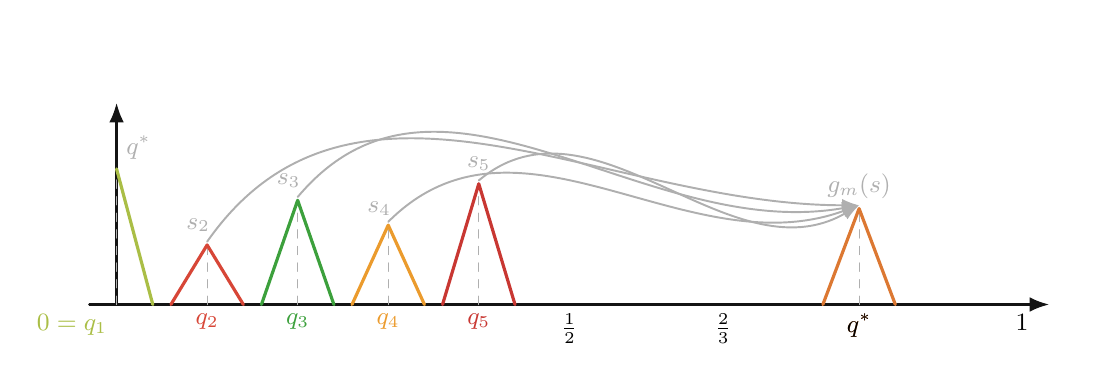
\begin{tikzpicture}[>=Latex, line cap=round, line join=round, font=\small, x=11.5cm, y=2.1cm]

% axis
\draw[->, line width=0.9pt, draw=nearblack] (-0.03,0) -- (1.03,0) node[below right] {};
\draw[->, line width=0.9pt, draw=nearblack] (0,0) -- (0,1.22);

% sample locations for the schematic N=6 example
\def\d{0.04}
\def\qone{0.00}
\def\qtwo{0.10}
\def\qthree{0.20}
\def\qfour{0.30}
\def\qfive{0.40}
\def\qstar{0.82}

% heights
\def\hone{0.82}
\def\htwo{0.36}
\def\hthree{0.63}
\def\hfour{0.48}
\def\hfive{0.73}
\def\hstar{0.58}

% guide lines
\draw[dashed, draw=lightgraytext] (\qone,0) -- (\qone,\hone);
\draw[dashed, draw=lightgraytext] (\qtwo,0) -- (\qtwo,\htwo);
\draw[dashed, draw=lightgraytext] (\qthree,0) -- (\qthree,\hthree);
\draw[dashed, draw=lightgraytext] (\qfour,0) -- (\qfour,\hfour);
\draw[dashed, draw=lightgraytext] (\qfive,0) -- (\qfive,\hfive);
\draw[dashed, draw=lightgraytext] (\qstar,0) -- (\qstar,\hstar);

% hats from the exact construction: q1 hat is clipped at the boundary, the others are standard hats
\draw[line width=1.15pt, draw=hatone] (\qone,\hone) -- ({\qone+\d},0);
\draw[line width=1.15pt, draw=hattwo] ({\qtwo-\d},0) -- (\qtwo,\htwo) -- ({\qtwo+\d},0);
\draw[line width=1.15pt, draw=hatthree] ({\qthree-\d},0) -- (\qthree,\hthree) -- ({\qthree+\d},0);
\draw[line width=1.15pt, draw=hatfour] ({\qfour-\d},0) -- (\qfour,\hfour) -- ({\qfour+\d},0);
\draw[line width=1.15pt, draw=hatfive] ({\qfive-\d},0) -- (\qfive,\hfive) -- ({\qfive+\d},0);
\draw[line width=1.15pt, draw=hatsix] ({\qstar-\d},0) -- (\qstar,\hstar) -- ({\qstar+\d},0);

% arrows showing that the fixed spikes determine the value stored at q^\ast
%\draw[->, line width=0.7pt, draw=lightgraytext] (\qone,\hone+0.02) to[out=55,in=170] (\qstar,0.02);
\draw[->, line width=0.7pt, draw=lightgraytext] (\qtwo,\htwo+0.02) to[out=55,in=180] (\qstar,\hstar+0.02);
\draw[->, line width=0.7pt, draw=lightgraytext] (\qthree,\hthree+0.02) to[out=50,in=190] (\qstar,\hstar+0.02);
\draw[->, line width=0.7pt, draw=lightgraytext] (\qfour,\hfour+0.02) to[out=45,in=200] (\qstar,\hstar+0.02);
\draw[->, line width=0.7pt, draw=lightgraytext] (\qfive,\hfive+0.02) to[out=40,in=210] (\qstar,\hstar+0.02);

% coefficient labels
\node[text=lightgraytext, above right] at (\qone,\hone) {$q^\ast$};
\node[text=lightgraytext, above] at (\qtwo-0.01,\htwo+0.02) {$s_2$};
\node[text=lightgraytext, above] at (\qthree-0.01,\hthree+0.02) {$s_3$};
\node[text=lightgraytext, above] at (\qfour-0.01,\hfour) {$s_4$};
\node[text=lightgraytext, above] at (\qfive,\hfive+0.02) {$s_5$};
\node[text=lightgraytext, above] at (\qstar,\hstar) {$g_m(s)$};

% support labels
\node[text=hatone, below left] at (\qone,0) {${0=q_1}$};
\node[text=hattwo, below] at (\qtwo,0) {${q_2}$};
\node[text=hatthree, below] at (\qthree,0) {${q_3}$};
\node[text=hatfour, below] at (\qfour,0) {${q_4}$};
\node[text=hatfive, below] at (\qfive,0) {${q_5}$};
\node[text=hatsix, below] at (\qstar,0) {${q^\ast}$};

% x-axis marks
\node[below] at (0.5,0) {$\frac12$};
\node[below] at (0.82,0) {$q^\ast$};
\node[below] at (0.67,0) {$\frac23$};
\node[below] at (1.00,0) {$1$};

\end{tikzpicture}
\caption{\textbf{Pointed-value family $\mathcal{T}_{N,m}^{\mathrm{val}}$.} A representative task from \eqref{eq:value-family} with $N = 6$ is shown. The fixed hats at $q_1,\dots,q_5$ carry the coefficients $q^\ast,s_2,\dots,s_5$ respectively, and the moving hat centered at $q^\ast\in[2/3,1]$ carries the value $g_m(s)$. 
%Note that the in-context learner can infer the position of the hat at $q^*$ from the sample at $q_1$. 
An unrestricted learner, whether in-context or agentic, can infer the position of the hat at $q^\ast$ by querying the task at the sample point $q_1$.
A general in-context learner can also derive the height of that hat, whereas a ReLU-based learner cannot. Both general and ReLU-based agentic learners can recover the height of the hat at $q^\ast$ by taking one sample.}
\label{fig:value-family}
\end{figure}
%

Fix $N\ge 3$ and a %ReLU 
weight budget $m\in\mathbb N$. 
Let $\delta >0$ be sufficiently small so that $\delta<1/(6N)$.
This choice guarantees that, for every $N$-point sample set, there exists a point in $[2/3,1]$ at distance greater than $\delta$ from all samples.
For every $a\in\mathbb{R}$, we define the hat function
\begin{equation} \label{hat}
    h_a(x)\eqdef  \bigg(1-\frac{|x-a|}{\delta}\bigg)_+.
\end{equation}
Let
\begin{equation} \label{theqs}
    q_i\eqdef  \frac{i-1}{2(N-1)},
    \qquad i=1,\dots,N,
\end{equation}
so that $0=q_1<q_2<\cdots<q_N=\frac12$. 
%Choose $\delta>0$ so small that the supports of the hats
%centerd at $q_1,\dots,q_N$ and at every point $q^\ast\in[2/3,1]$ are pairwise disjoint, with in addition $\delta<1/(6N)$, which guarantees that every $N$-point sample set leaves some point of $[2/3,1]$ at distance greater than $\delta$ from all samples; this is used in the lower-boundarguments below. 

%For every $a\in\mathbb{R}$, define
%\[
    %h_a(x)\eqdef  \bigg(1-\frac{|x-a|}{\delta}\bigg)_+.
%\]
Choose a continuous hard function
$
g_m:[0,1]^{N-2}\to[0,1]
$
such that every ReLU network with at most $m$ weights has uniform approximation error at least
$1/2$ on $g_m$. This function exists according to Remark \ref{rem:unattainableFunctions}.
For $s=(s_2,\dots,s_{N-1})\in[0,1]^{N-2}$ and
$q^\ast\in[2/3,1]$, define the task
\begin{equation}
\label{eq:value-family}
f^{\mathrm{val}}_{s,q^\ast}(x)
\eqdef 
q^\ast h_{q_1}(x)+\sum_{i=2}^{N-1} s_i h_{q_i}(x)+g_m(s)h_{q^\ast}(x).
\end{equation}
By construction, the supports of the hat functions centered at $q_1,\dots,q_N$ are pairwise disjoint. We depict one example in Figure~\ref{fig:value-family}.
Moreover, for each $i$, the support of the hat function at $q_i$ is disjoint from that at $q^\ast\in [2/3,1]$, with separation at least $1/6-2\delta>0$.
Let $\mathcal{T}_{N,m}^{\mathrm{val}}$ denote the resulting \emph{pointed-value} task family of all such $f^{\mathrm{val}}_{s,q^\ast}$.


\begin{theorem}
\label{thm:value}
Let $\eta >0$ and $N \in \mathbb N$ with $N\geq 3$. For sufficiently large $m \in \mathbb N$ depending only on N and $\eta$ the following hold for the family $\mathcal{T}_{N,m}^{\mathrm{val}}$:
\begin{enumerate}
    \item[\rm (i)] Unrestricted in-context learning reconstructs every task exactly from the fixed %context 
    query points $\{q_1,\dots,q_N\}$.
    \item[\rm (ii)] Unrestricted agentic learning also reconstructs every task exactly with a query budget $N$.
    \item[\rm (iii)] Every ReLU-realizable in-context learner with a sample budget $N$ and a weight budget $m$ %with at most $m$ weights 
    incurs worst-case
    $L^\infty([0,1])$ approximation error at least $1/2$. 
    \item[\rm (iv)] There exists a ReLU-realizable agentic learner, with a query budget $N$ and a weight budget $m$, %size $m$ 
    whose worst-case $L^\infty([0,1])$ approximation error on $\mathcal{T}_{N,m}^{\mathrm{val}}$ is at most
    \(\eta\).
\end{enumerate}
Consequently, for \(\eta<1/2\) and $m$ sufficiently large, %Definition~\ref{def:formalDefRelations} gives
\[
\ICG=\AG
\quad\text{ and }\quad
\ICR<\AR.
\]
\end{theorem}

The proof of Theorem~\ref{thm:value} can be founded in Appendix~\ref{appx:pointedvalue}.

We briefly summarize the main idea of the construction \eqref{eq:value-family}, which underlies the proof.
%The mechanism is the dual of the next section. 
Here the hard object is the \emph{value}
$g_m(s)$, but it is placed at an accessible %easy-to-find 
location $q^\ast$, which can be read directly from the initial contexts (e.g., via $f^{\mathrm{val}}_{s,q^\ast}(q_1)$). 
Unrestricted in-context
and agentic learning are equally powerful because both can compute $g_m(s)$ once $s$ is obtained from the context (e.g., via $f^{\mathrm{val}}_{s,q^\ast}(q_i)$). %from the context. 
An illustration of this process is given in Figure~\ref{fig:value-family}.
Under ReLU realizability, however, a non-adaptive predictor must approximate the hard map $s\mapsto g_m(s)$ internally, whereas a ReLU-realizable agentic learner can query this value $g_m(s)$
directly and %then use standard ReLU approximate multiplication to 
reconstruct the %corresponding
task $f^{\mathrm{val}}_{s,q^\ast}$ using classical ReLU approximation.
%spike expansion to arbitrary accuracy.



\subsection{Information advantage blocked by realizability}
\label{s:Main__ss:killed-by-realizability}

\begin{figure}[htb]
\centering
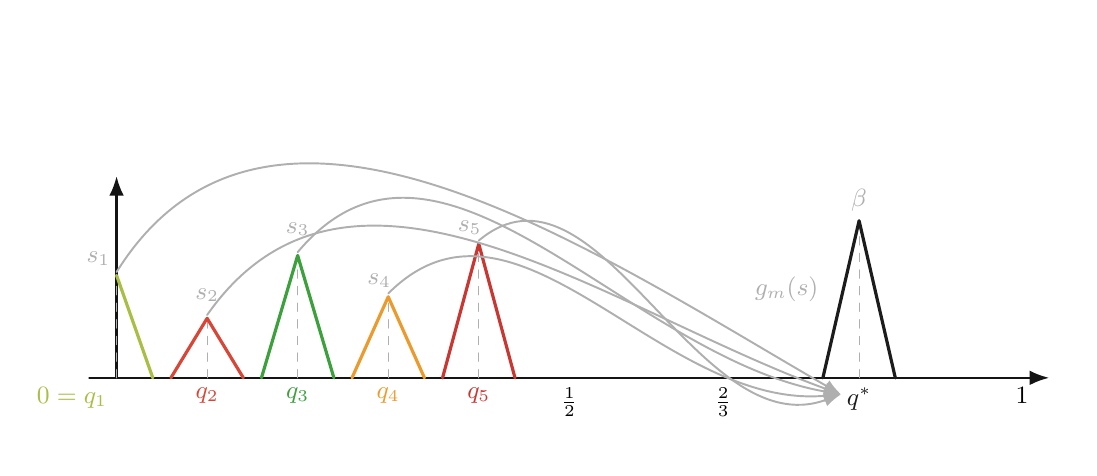
\begin{tikzpicture}[>=Latex, line cap=round, line join=round, font=\small, x=11.5cm, y=2.1cm]

% axis
\draw[->, line width=0.9pt, draw=nearblack] (-0.03,0) -- (1.03,0) node[below right] {};
\draw[->, line width=0.9pt, draw=nearblack] (0,0) -- (0,1.22);

% sample locations for a schematic with six fixed hats and one moving hat
\def\d{0.04}
\def\qone{0.00}
\def\qtwo{0.10}
\def\qthree{0.20}
\def\qfour{0.30}
\def\qfive{0.40}
\def\qsix{0.50}
\def\qstar{0.82}

% heights
\def\hone{0.62}
\def\htwo{0.36}
\def\hthree{0.74}
\def\hfour{0.49}
\def\hfive{0.81}
\def\hsix{0.58}
\def\hstar{0.95}

% guide lines
\draw[dashed, draw=lightgraytext] (\qone,0) -- (\qone,\hone);
\draw[dashed, draw=lightgraytext] (\qtwo,0) -- (\qtwo,\htwo);
\draw[dashed, draw=lightgraytext] (\qthree,0) -- (\qthree,\hthree);
\draw[dashed, draw=lightgraytext] (\qfour,0) -- (\qfour,\hfour);
\draw[dashed, draw=lightgraytext] (\qfive,0) -- (\qfive,\hfive);
\draw[dashed, draw=lightgraytext] (\qstar,0) -- (\qstar,\hstar);

% hats from the exact construction: q1 hat is clipped at the boundary, the others are standard hats
\draw[line width=1.15pt, draw=hatone] (\qone,\hone) -- ({\qone+\d},0);
\draw[line width=1.15pt, draw=hattwo] ({\qtwo-\d},0) -- (\qtwo,\htwo) -- ({\qtwo+\d},0);
\draw[line width=1.15pt, draw=hatthree] ({\qthree-\d},0) -- (\qthree,\hthree) -- ({\qthree+\d},0);
\draw[line width=1.15pt, draw=hatfour] ({\qfour-\d},0) -- (\qfour,\hfour) -- ({\qfour+\d},0);
\draw[line width=1.15pt, draw=hatfive] ({\qfive-\d},0) -- (\qfive,\hfive) -- ({\qfive+\d},0);
\draw[line width=1.15pt, draw=charcoalblack] ({\qstar-\d},0) -- (\qstar,\hstar) -- ({\qstar+\d},0);

% arrows showing that the fixed spike values determine the location q^\ast
\draw[->, line width=0.7pt, draw=lightgraytext] (\qone,\hone+0.02) to[out=58,in=150] (\qstar-0.02,-0.1);
\draw[->, line width=0.7pt, draw=lightgraytext] (\qtwo,\htwo+0.02) to[out=55,in=160] (\qstar-0.02,-0.1);
\draw[->, line width=0.7pt, draw=lightgraytext] (\qthree,\hthree+0.02) to[out=50,in=170] (\qstar-0.02,-0.1);
\draw[->, line width=0.7pt, draw=lightgraytext] (\qfour,\hfour+0.02) to[out=45,in=185] (\qstar-0.02,-0.1);
\draw[->, line width=0.7pt, draw=lightgraytext] (\qfive,\hfive+0.02) to[out=40,in=200] (\qstar-0.02,-0.1);

% coefficient labels
\node[text=lightgraytext, above] at (\qone-0.02,\hone) {$s_1$};
\node[text=lightgraytext, above] at (\qtwo,\htwo+ 0.04) {$s_2$};
\node[text=lightgraytext, above] at (\qthree,\hthree+0.06) {$s_3$};
\node[text=lightgraytext, above] at (\qfour-0.01,\hfour) {$s_4$};
\node[text=lightgraytext, above] at (\qfive-0.01,\hfive) {$s_5$};
\node[text=lightgraytext, above] at (\qstar,\hstar) {$\beta$};
\node[text=lightgraytext, above] at (\qstar-0.08,0.4) {$g_m(s)$};

% support labels
\node[text=hatone, below left] at (\qone,0) {${0=q_1}$};
\node[text=hattwo, below] at (\qtwo,0) {${q_2}$};
\node[text=hatthree, below] at (\qthree,0) {${q_3}$};
\node[text=hatfour, below] at (\qfour,0) {${q_4}$};
\node[text=hatfive, below] at (\qfive,0) {${q_5}$};
\node[text=charcoalblack, below] at (\qstar,0) {${q^\ast}$};

% x-axis marks
\node[below] at (0.5,0) {$\frac12$};
\node[below] at (0.67,0) {$\frac23$};
\node[below] at (1.00,0) {$1$};

\end{tikzpicture}
\caption{\textbf{Address-spike family $\mathcal{T}_{N,m}^{\mathrm{addr}}$.} A representative task from \eqref{eq:addrtasks} for $N = 6$ is shown: the coefficients at $q_1,\dots,q_5$ are respectively $s_1,\dots,s_5$, and these values determine the moving location $q^\ast(s)\in[2/3,1]$. The moving hat centered at $q^\ast(s)$ carries a hidden bit $\beta$. We show that no in-context learner can reliably identify the value of $\beta$, and the same is true for a ReLU-based agentic learner. A general agent, however, can compute $q^\ast$ from the samples at $q_1,\dots,q_5$ and then take one additional sample that reveals $\beta$.}
\label{fig:address_spike}
\end{figure}
%\footnotetext{The same obstruction holds for any neural network agent class with finite $\gamma$-fat-shattering dimension, for sufficiently small scale parameter $\gamma>0$.}





%The third pattern is complementary. Unrestricted adaptivity still helps, but only because the agent
%can compute the informative query location. Once the query location itself must be produced by a
%bounded-size ReLU controller, the advantage of adaptivity can disappear. 
% We now exhibit this phenomenon:


Our third family of tasks is complementary to the second considered in the previous section. 
This family shows that adaptivity can disappear under realizability constraints.

Fix again $N\ge 3$ and $m\in\mathbb N$, with the same points $q_1,\dots,q_N$ in \eqref{theqs}. % and the hat functions $h_a$ of the previous section. 
Let
$
\tau(t)\eqdef 2\min\{t,1-t\},
$ for each $t\in[0,1]$, 
and write for $s=(s_1,\dots,s_{N-1})\in[0,1]^{N-1}$
\begin{equation} \label{hats}
    \widehat s\eqdef  (\tau(s_1),\dots,\tau(s_{N-1})).
\end{equation}
Choose a continuous hard-to-approximate surjective map
$
g_m:[0,1]^{N-1}\to\left[\frac23,1\right]
$
such that every ReLU network with at most $m$ weights has uniform approximation error at least
$1/6$ on $g_m$. Such a function exists by Remark~\ref{rem:unattainableFunctions}. Moreover, since any such hard function is non-constant, one may apply an affine rescaling of its image to ensure surjectivity onto $[2/3,1]$ without decreasing the approximation hardness. 
For $s=(s_1,\dots,s_{N-1})\in[0,1]^{N-1}$ and $\beta\in\{0,1\}$, define
$
q^\ast(s)\eqdef g_m(\widehat s)
$
and
\begin{equation} \label{eq:addrtasks}
    f^{\mathrm{addr}}_{s,\beta}(x)
    \eqdef 
    \sum_{i=1}^{N-1} s_i h_{q_i}(x)
    +
    \beta h_{q^\ast(s)}(x),
\end{equation}
where the hat functions $h_a$ are given in \eqref{hat} with $\delta<1/(6N)$.
Let \(\mathcal T_{N,m}^{\mathrm{addr}}\) denote the resulting \emph{address-spike} family of all such $f^{\mathrm{addr}}_{s,\beta}$. We depict one example of a function in \(\mathcal T_{N,m}^{\mathrm{addr}}\) in Figure \ref{fig:address_spike}.

\begin{theorem}
\label{thm:address}
Let $m,N\in\mathbb{N}$ with $N\geq 3$.
For the family $\mathcal{T}_{N,m}^{\mathrm{addr}}$, the following hold.
\begin{enumerate}
    \item[\rm (i)] %There exists a general agentic learner that first reads the static values at
    %$q_1,\dots,q_{N-1}$ and then makes one additional adaptive query, reconstructing every task exactly.
    There exists a general agentic learner with a query budget $N$ consisting of $N-1$ fixed queries followed by one adaptive query, that reconstructs every task exactly.
    \item[\rm (ii)] Every in-context learner with the sample budget $N$ incurs worst-case
    $L^\infty([0,1])$ approximation error at least $1/2$.
    \item[(iii)] Every ReLU-realizable agentic learner with query budget \(N\) and query maps implemented by ReLU networks with at most $m$ weights incurs worst-case 
    \(L^\infty([0,1])\) approximation error at least \(1/2\). 
\end{enumerate}
Consequently, 
\begin{equation*}
    \ICG<\AG \quad\text{ and }\quad \ICR=\AR.
\end{equation*}
%Part~\textup{(i)} together with part~\textup{(ii)} yields $\ICG<\AG$. Part~\textup{(iii)} $\ICR = \AR$ since the worst-case error 1/2 can be achieved by a constant approximator.
\end{theorem}

The proof of Theorem~\ref{thm:address} is given in Appendix~\ref{appx:address}

We now briefly summarize the main idea of the construction \eqref{eq:addrtasks}, which underlies the proof.
The mechanism here dual to that in the previous section. 
The hard object here is the \emph{location} $q^\ast(s)$ itself. Unrestricted adaptivity helps,
because after reading the static coefficients the learner %one 
can compute $q^\ast(s)$ and then query $f^{\mathrm{addr}}_{s,\beta}$ there to learn the hidden bit $\beta$. 
An illustration of this process is given Figure~\ref{fig:address_spike}.
%But bounded-size ReLU adaptivity does not help: 
However, under ReLU realizability, this advantage changes.
Finding the informative query point
already requires approximating the hard map $s\mapsto q^\ast(s)=g_m(\widehat s)$. Therefore, query maps %controller inherits 
face the
same obstruction as %the non-adaptive ReLU predictor
an in-context learner. 



\section*{Acknowledgements}

A.M.N. and P.C.P. were %are 
supported by the Austrian Science Fund (FWF) Project P-37010.

\newpage
\bibliographystyle{acm}
\bibliography{Bookkeeping/bibibib}



\appendix

\section{Deep learning models}
\label{s:models}

%For completeness, we briefly review the deep learning models considered in this paper. 
For completeness, we briefly recall the relevant deep learning models.
 

\begin{definition}[Fully connected MLPs]
Let $d,D,L\in\mathbb{N}$, and let $d_0,d_1,\dots,d_L\in\mathbb{N}$ such that $d_0=d$ and $d_L=D$.
Let $\sigma\in \mathcal{C}(\mathbb{R})$ be an activation function.
A fully-connected MLP with depth $L$ and activation function $\sigma$ is a map $f:\mathbb{R}^d\to\mathbb{R}^D$ with iterative representation:
\begin{align*} %\label{eq:representation_MLP}
    &X^{(0)} 
    \eqdef  X, \\
    &X^{(j+1)} 
    \eqdef  
    \sigma\bullet({\bf A}^{(j)} X^{(j)} + b^{(j)}) \qquad j=0,1,\dots,L-2,
    \qquad f(X)
    \eqdef  
    {\bf A}^{(L-1)} X^{(L-1)} + b^{(L-1)},
\end{align*}
where $\bullet$ denotes component-wise application, ${\bf A}^{(j)}\in\mathbb{R}^{d_{j+1}\times d_j}$, and $b^{(j)}\in\mathbb{R}^{d_{j+1}}$.
%Here, $J$ is the depth of the MLP and $\Upsilon\eqdef  \max_{j=1,\dots,J-1}\,d_j$ is its width.
\end{definition}





\begin{definition}[Transformers with multi-head attention]
%Fix a temperature parameter $\lambda>0$ and dimensions $d_{\rm in},d_{{\rm key}},d_{\rm out},N\in \mathbb N$.  
Let $\lambda>0$, and let $d_{\rm in},d_{{\rm key}},d_{\rm out},N\in \mathbb N$. 
Let
${\bf Q},{\bf K}\in \mathbb{R}^{d_{{\rm key}}\times d_{\rm in}}$
and
${\bf V}\in \mathbb{R}^{d_{\rm out}\times d_{\rm in}}$. 
We define the associated attention mechanism
$\operatorname{Attn}(\cdot|{\bf Q},{\bf K},{\bf V},\lambda):\mathbb{R}^{N\times d_{\rm in}}\to \mathbb{R}^{N\times d_{\rm out}}
$
by
\begin{equation} \label{eq:def_attention}
    [\operatorname{Attn}(\mathbf{X}|{\bf Q},{\bf K},{\bf V},\lambda)]_n
    \eqdef 
    \sum_{m=1}^N
    \frac{e^{\lambda \langle {\bf Q}[\mathbf{X}]_n, {\bf K}[\mathbf{X}]_m\rangle/\sqrt{d_{{\rm key}}}}}{
    \sum_{l=1}^N e^{\lambda \langle {\bf Q}[\mathbf{X}]_n, {\bf K}[\mathbf{X}]_l \rangle/\sqrt{d_{{\rm key}}}}}
    {\bf V}[\mathbf{X}]_m, \qquad n=1,\dots,N.
\end{equation}
Here $[\mathbf{X}]_j \in \mathbb{R}^{d_{\rm in}}$ denotes the $j$th row of $\mathbf{X}$, interpreted as a column vector when multiplied by ${\bf Q},{\bf K},{\bf V}$.
%A transformer network operates by iteratively applying row-wise activation-bias maps and then applying attention mechanisms matrix-wise.  
A transformer network operates by iterating layers, each consisting of a row-wise activation–bias map followed by an attention mechanism.
Concretely, let $d,D,L\in\mathbb{N}$, and let $d_0,d_1,\dots,d_L, H_0,H_1,\dots,H_L\in\mathbb{N}$ such that $d_0=d$ and $d_L=D$.
For $j=0,1,\dots,L-2$ and $\mathtt{h}=1,\dots,H_j$, let $d^{(j)}_{{\rm key}, \mathtt{h}}, d^{(j)}_{{\rm value}, \mathtt{h}}\in\mathbb{N}$ such that $d_{j+1} = \sum_{{\mathtt{h}}=1}^{H_j} d^{(j)}_{{\rm value}, \mathtt{h}}$.
A $j$th \emph{transformer layer with multi-head attention}, for $j=0,1,\dots,L-2$, is a map
$
\mathcal{T}_j:\mathbb{R}^{N\times d_j}\to \mathbb{R}^{N\times d_{j+1}}
$
that sends an input matrix $\mathbf{X}^{(j)}\in \mathbb{R}^{N\times d_j}$ to
$
\mathcal{T}_j(\mathbf{X}^{(j)})\eqdef  \mathbf{X}^{(j+1)}\in \mathbb{R}^{N\times d_{j+1}},
$
where 
\begin{alignat}{2} %\label{eq:representation_transformer}
    \nonumber \mathbf{Z}^{(j)}
    &\eqdef 
    \underbrace{
        \bigoplus_{\mathtt{h}=1}^{H_j}
            \operatorname{Attn}\big(
                \mathbf{X}^{(j)}
                |{\bf Q}_{\mathtt{h}}^{(j)},{\bf K}_{\mathtt{h}}^{(j)},{\bf V}_{\mathtt{h}}^{(j)},\lambda
            \big)
    }_{\text{multi-head attention}} && \\
    \label{eq:representation_transformer} [\mathbf{X}^{(j+1)}]_n
    &\eqdef  
    %\underbrace{
        \sigma\bullet
        \big(
            [\mathbf{Z}^{(j)}]_n + b^{(j)}
        \big),
    %}_{\text{Activation and Bias}},
    &&\qquad n=1,\dots,N.
\end{alignat}
Here $\bigoplus$ denotes concatenation along the second (column) dimension, $
{\bf Q}_{\mathtt{h}}^{(j)},{\bf K}_{\mathtt{h}}^{(j)}\in \mathbb{R}^{d_{{\rm key}, \mathtt{h}}^{(j)}\times d_j}$ and 
$
{\bf V}_{\mathtt{h}}^{(j)}\in \mathbb{R}^{d_{{\rm value}, \mathtt{h}}^{(j)}\times d_j}$, and $b^{(j)}\in\mathbb{R}^{d_{j+1}}$.
Further, the addition in \eqref{eq:representation_transformer} is applied row-wise.
A \emph{transformer with multi-head attention} with depth $L$, obtained by composing the layers $\mathcal{T}_0,\mathcal{T}_1,\dots,\mathcal{T}_{L-2}$, is a map $\mathcal{T}:\mathbb{R}^{N\times d}\to\mathbb{R}^{N\times D}$ sending an input matrix ${\bf X}^{(0)}\eqdef {\bf X}\in\mathbb{R}^{N\times d}$ to $\mathcal{T}({\bf X}) \eqdef {\bf A}^{(L-1)}{\bf X}^{(L-1)} + b^{(L-1)}\in\mathbb{R}^{N\times D}$, for some ${\bf A}^{(L-1)}\in\mathbb{R}^{D\times d_{L-1}}$ and $b^{(L-1)}\in\mathbb{R}^D$.
%Here, $J$ is called the depth of the transformer, $\max_{j=0,\dots,J-1}H_j$ is the maximum number of attention heads, and $\max_{j=1,\dots,J-1}d_j$ is called its width.
\end{definition}


Similar to the strategy of~\cite{petersen2020equivalence}, we 
show that every ReLU MLP can be converted into a transformer in a canonical fashion. 
This allows us to deduce a quantitative version of the in-context universality results of~\cite{furuya2025transformers} for the transformer model. 
The next result is the analogue of~\cite[Proposition 11]{kratsios2025context} for our formulation of the transformer used here. 




% \begin{proposition}[Transformerification of MLPs]
% \label{prop:transformerification__SparseVersion}
% Let $f:\mathbb{R}^d\to \mathbb{R}^D$ be a $\sigma$-MLP with depth $J$, width $W$, and size $K$; $J,W,K\in \mathbb N$.  
% Then, for every $\lambda>0$, $f$ can be implemented exactly as a one-token transformer with the same depth and width as $f$, exactly one attention head at each layer, and at most $K$ non-zero trainable affine parameters.
% \end{proposition}

\begin{proposition}[Transformerification of MLPs]
\label{prop:transformerification__SparseVersion}
Let $f:\mathbb{R}^d\to \mathbb{R}^D$ be a MLP with depth $L$. %, width $W$, and size $K$, where $J,W,K\in \mathbb N$.  
Then, for every $\lambda>0$, $f$ can be implemented exactly as a %one-token 
transformer with the same depth %and width 
as $f$, exactly one attention head at each layer. %, and at most $K$ non-zero trainable affine parameters.
\end{proposition}

\begin{proof}[{Proof of Proposition~\ref{prop:transformerification__SparseVersion}}]
Let $d_0,d_1,\dots,d_L\in\mathbb{N}$ such that $d_0=d$ and $d_L=D$.
Let $f:\mathbb{R}^d\to\mathbb{R}^D$ admit the iterative representation
\begin{equation}
\label{eq:representation_MLP_}
    \begin{aligned}
    f(X)
    & \eqdef  
    {\bf A}^{(L-1)} X^{(L)}+b^{(L-1)}
    \\
    X^{(j+1)} 
    &
    \eqdef  
    \sigma\bullet\big(
        {\bf A}^{(j)}X^{(j)}
            +
        b^{(j)}
    \big)
    \qquad 
            \mbox{for }  
        j=0,1,\dots,L-2,    
    \\
    X^{(0)} &\eqdef X,
    \end{aligned}
\end{equation}
where ${\bf A}^{(j)}\in\mathbb{R}^{d_{j+1}\times d_j}$ and $b^{(j)}\in\mathbb{R}^{d_{j+1}}$.
Identify each $X^{(j)}\in\mathbb{R}^{d_j}$ with the matrix
$\mathbf{X}^{(j)}\in\mathbb{R}^{1\times d_j}$ whose unique row is $X^{(j)}$.
For each $j=0,1,\dots,L-2$, we define
\[
    {\bf Q}^{(j)}\eqdef  0\in\mathbb{R}^{1\times d_j},
    \qquad
    {\bf K}^{(j)}\eqdef  0\in\mathbb{R}^{1\times d_j},
    \qquad
    {\bf V}^{(j)}\eqdef  {\bf A}^{(j)}\in\mathbb{R}^{d_{j+1}\times d_j}.
\]
%Since there is only one token, the unique attention weight is equal to $1$.  
It follows from \eqref{eq:def_attention} that for every $\lambda>0$,
$\operatorname{Attn}(\mathbf{X}^{(j)} \mid {\bf Q}^{(j)},{\bf K}^{(j)},{\bf V}^{(j)},\lambda)$ is a matrix with a single row:
\[
    [\operatorname{Attn}(
        \mathbf{X}^{(j)}
        |{\bf Q}^{(j)},{\bf K}^{(j)},{\bf V}^{(j)},\lambda
    )]_1
    =
    {\bf A}^{(j)} {\bf X}^{(j)}.
\]
Therefore, the transformer recursion
\begin{align*} 
    \mathbf{X}^{(j+1)}
    &\eqdef 
    \sigma\bullet \big(
        \operatorname{Attn}(
            \mathbf{X}^{(j)}
            |{\bf Q}^{(j)},{\bf K}^{(j)},{\bf V}^{(j)},\lambda
        )
        +
        b^{(j)}
    \big) 
    \qquad j=0,1,\dots,L-2,
    \\
    \mathbf{X}^{(0)}
    &\eqdef  X,
\end{align*}
satisfies
$
\mathbf{X}^{(j)}=X^{(j)}
$
for every $j=0,1,\dots,L-1$.  
The final affine map can be implemented in the same way, by taking
\[
    {\bf Q}^{(L-1)}\eqdef  0\in\mathbb{R}^{1\times D},
    \qquad
    {\bf K}^{(L-1)}\eqdef  0\in\mathbb{R}^{1\times D},
    \qquad
    {\bf V}^{(L-1)}\eqdef  {\bf A}^{(L-1)}\in\mathbb{R}^{D\times d_{L-1}},
\]
and setting
\[
    \mathcal{T}(X)
    \eqdef 
    \operatorname{Attn}(
        \mathbf{X}^{(L)}
        |{\bf Q}^{(L)},{\bf K}^{(L)},{\bf V}^{(L)},\lambda
    )
    +
    b^{(L)}
    =
    {\bf A}^{(L)}X^{(L)}+b^{(L)}
    =
    f(X).
\]
Thus, we conclude that the designed transformer implements $f$ exactly, with unchanged depth $L$.
%Moreover, the only non-zero trainable parameters of the constructed transformer are precisely the entries of the matrices ${\bf A}^{(j)}$ and biases $b^{(j)}$, while all query and key matrices are fixed to zero.  
%Hence the transformer has at most $K$ non-zero trainable affine parameters.  
%This concludes the proof.
\end{proof}

\section{Approximate multiplication by ReLU neural networks}

For convenience, we recall a standard result on approximating multiplication.


\begin{lemma}[{\cite[Proposition 3]{yarotsky2017}}]
\label{lem:approx-mult}
For every \(\varepsilon\in(0,1)\) there exists a ReLU network
\[
\operatorname{Mult}_{\varepsilon}:[0,1]^2\to[0,1]
\]
with \(\mathcal{O}(\log(1/\varepsilon))\) weights such that
$
\sup_{a,b\in[0,1]}
\left|
\operatorname{Mult}_{\varepsilon}(a,b)-ab
\right|
\leq \varepsilon 
$.
\end{lemma}


\section{Proof of Theorem~\ref{thm:path}}
\label{appx:cubicalpath}



\begin{lemma}[Exact ReLU realization of a cubical bump]
\label{lem:cubical-bump}
For every $d,n\in\mathbb N$ and every cube $Q\in\mathcal Q_n$, the bump $\theta_Q$ is exactly
representable by a ReLU network of size and depth $\mathcal O(d)$, with hidden constants depending only
on $\eta$.
\end{lemma}

\begin{proof}
Using the standard exact identities
\[
|u|=\ReLU(u)+\ReLU(-u),
\qquad
\max\{a,b\}=\ReLU(a-b)+b,
\]
one obtains an exact ReLU realization of the coordinatewise maximum
\[
M_d(z_1,\dots,z_d)\eqdef \max\{z_1,\dots,z_d\}
\]
with size and depth $\mathcal O(d)$. 
Moreover, if $Q\in\mathcal Q_n$ has the center $c=(c_1,\dots,c_d)$ and
side length $\ell(Q)=2^{-n}$, then by definition~\eqref{centralcube},
\[
\operatorname{dist}_{\infty}(x,Q_\eta)
=
\max_{i\in[d]}\bigl(|x_i-c_i|-\eta\ell(Q)\bigr)_+.
\]
Hence
\[
\theta_Q(x)
=
\Bigg(
1-
\frac{1}{(\tfrac12-\eta)\ell(Q)}
M_d\Big(\bigl(|x_i-c_i|-\eta\ell(Q)\bigr)_+\Big)_{i=1}^d
\Bigg)_+.
\]
This last expression is built from affine maps, absolute values, maxima, and two extra ReLUs; %one final ReLU, so it is
therefore, $\theta_Q$ is exactly ReLU-realizable with the stated network size and depth. %complexity.
\end{proof}

We denote by $\Theta(c,\cdot)$ (or $\Theta(c(Q),\cdot)$) the ReLU realization of the bump from Lemma~\ref{lem:cubical-bump}, emphasizing its dependence on the center $c$, in accordance with the translation-invariance of the construction.

\begin{proof}[Proof of Theorem~\ref{thm:path}]
Write $K\eqdef  2^d$ and fix an enumeration $\varepsilon^1,\dots,\varepsilon^K$ of $\{-1,+1\}^d$. 
We construct a ReLU-realizable agentic learner $\Psi$ using $K$ queries per level, hence
$KL=2^dL$ queries in total.
The learner $\Psi$ stores the recovered cube centers level by level. Initialize with the center of
$[0,1]^d$, which is the unique level-$0$ cube. Suppose the center $c^{(n-1)}$ of the path cube at
level $n-1$ has already been recovered. The $K$ dyadic children of that cube have centers
\[
q_j=c^{(n-1)}+2^{-(n+1)}\varepsilon^j,
\qquad j=1,\dots,K.
\]
These query points $q_j$ are affine functions in the current %state, 
transcript $c^{(n-1)}$ and therefore are ReLU-realizable. 
The $K$ queries are performed sequentially: the learner $\Psi$ queries the points $q_j$ one by one, evaluating the task at each %and let $y_j=f^\Gamma(q_j)$ denote the responses.
and recording the response $y_j=f^{\Gamma}(q_j)$. 
Subtract the contribution of the previously recovered ancestor bumps and define the residuals 
\[
\rho_j
\eqdef 
y_j-\sum_{l=1}^{n-1}\Theta_l(c^{(l)},q_j),
\qquad j=1,\dots,K,
\]
where $\Theta_l$ is the ReLU network from Lemma~\ref{lem:cubical-bump} realizing a level $l$ bump
from its center. Exactly one residual equals $1$, namely the one corresponding to the true child on
the hidden path. Indeed, the level $n$ bump function $\theta_{Q^{(n)}}$ equals $1$ at the center of its own cube and $0$ at
the centers of the other children. 
Moreover, since $\eta\in (0,1/2)$, every deeper bump vanishes at the centers of the level $n$ children. Thus
\[
\rho_j=
\begin{cases}
1 &\text{ if }q_j=c(Q^{(n)}),\\
0 &\text{ otherwise.}
\end{cases}
\]
Using
\[
\chi(t)\eqdef  \ReLU(t)-\ReLU(t-1),
\]
which satisfies $\chi(0)=0$ and $\chi(1)=1$, the new center of the path cube at level $n$ is recovered by the ReLU formula
\[
c^{(n)}\eqdef\sum_{j=1}^K \chi(\rho_j)q_j.
\]
Putting these observations together, we conclude that all the query maps are %the state update is 
ReLU-realizable.
After $L$ levels, the learner $\Psi$ knows $c^{(1)},\dots,c^{(L)}$ and outputs
\begin{equation} \label{finalpred}
    \widehat{F}_{\Psi}(x)\eqdef\sum_{n=1}^L \Theta_n(c^{(n)},x).
\end{equation}
By the construction, $c^{(n)}=c(Q^{(n)})$ for every $n$, so $\widehat{F}_{\Psi}(x)=f^\Gamma(x)$ for all $x\in[0,1]^d$.
It follows from \eqref{finalpred} and Lemma~\ref{lem:cubical-bump} that $\widehat{F}_{\Psi}$ is ReLU-realizable. 
This proves part~(i). 


For part~(ii), let us consider %a non-adaptive 
an in-context learner $\Psi$ using $N<2^{d(L-1)}$ query points $(x_i)_{i=1}^N$.
The dyadic partition $\mathcal Q_{L-1}$ has exactly $2^{d(L-1)}$ cubes, so some cube $Q\in\mathcal Q_{L-1}$ contains no query point. 
Let $Q_1,Q_2$ be two distinct children of $Q$ at level $L$.
Let $\Gamma_1 = (Q^{(1)},\dots,Q^{(L-1)}, Q^{(L)}_1\}$ and $\Gamma_2 = (Q^{(1)},\dots,Q^{(L-1)}, Q^{(L)}_2\}$ be two cubical paths of length $L$ where $Q^{(L-1)}=Q$, and $Q^{(L)}_1=Q_1$, $Q^{(L)}_2=Q_2$.
%Choose a common path prefix ending at $Q$, and let $Q_1,Q_2$ be two distinct children of $Q$ at level $L$. The corresponding tasks $f^{\Gamma_1}$ and $f^{\Gamma_2}$ agree on every query point, since they differ only in the final bump supported inside $Q$. 
Recalling definition~\eqref{eq:cubical_path}, the associated tasks $f^{\Gamma_1}, f^{\Gamma_2}\in \mathcal{T}_{d,L}^{\mathrm{path}}$ on $N<2^{d(L-1)}$ query points yield the same context:
\begin{equation*}
    C_N(f^{\Gamma_1};x_1,\dots,x_N) = ((x_i,f^{\Gamma_1}(x_i)))_{i=1}^N
    = ((x_i,f^{\Gamma_2}(x_i)))_{i=1}^N =C_N(f^{\Gamma_2};x_1,\dots,x_N).
\end{equation*}
Since the learner $\Psi$ depends only on this context, it produces the same approximation for both tasks, i.e. $\Psi(f^{\Gamma_1})=\Psi(f^{\Gamma_2})$.
%Therefore the learner produces the same approximation for both tasks. 
Now let $z=c(Q_1)$. Then $\theta_{Q_1}(z)=1$ and $\theta_{Q_2}(z)=0$; hence %while all coarser bumps are identical, so
\[
|f^{\Gamma_1}(z)-f^{\Gamma_2}(z)|=1,
\]
which implies
\begin{equation} \label{thingtocontradict}
    \|f^{\Gamma_1}-f^{\Gamma_2}\|_{L^\infty([0,1]^d)}\ge 1.
\end{equation}
Suppose that
\begin{equation} \label{impossibility}
    \|\Psi(f^{\Gamma_i})-f^{\Gamma_i}\|_{L^\infty([0,1]^d)} < 1/2 \qquad i=1,2.
\end{equation}
Then 
\begin{align*}
    \|f^{\Gamma_1}-f^{\Gamma_2}\|_{L^\infty([0,1]^d)} &\leq \|\Psi(f^{\Gamma_1})-f^{\Gamma_1}\|_{L^\infty([0,1]^d)} + \|\Psi(f^{\Gamma_1})-f^{\Gamma_2}\|_{L^\infty([0,1]^d)} \\
    &= \|\Psi(f^{\Gamma_1})-f^{\Gamma_1}\|_{L^\infty([0,1]^d)} + \|\Psi(f^{\Gamma_2})-f^{\Gamma_2}\|_{L^\infty([0,1]^d)} < 1,
\end{align*}
%If one common approximation were within error $<1/2$ of both tasks, the triangle inequality would give $\|f^{\Gamma_1}-f^{\Gamma_2}\|_{L^\infty}<1$, a contradiction. 
contradicting \eqref{thingtocontradict}.
Thus at least one of the two tasks incurs an approximation error at least $1/2$ from $\Psi$ in \eqref{impossibility}. 
Since $\Psi$ is an arbitrary in-context learner, it follows that any in-context learner using $N<2^{d(L-1)}$ queries must incur worst-case $L^\infty([0,1]^d)$ approximation error at least $1/2$ on the task family $\mathcal{T}_{d,L}^{\mathrm{path}}$. This proves part~(ii).

%Part~(i) gives exact reconstruction in both $\AG$ and $\AR$. Combined with part~(ii), this yields the strict comparisons stated in Theorem~\ref{thm:path} whenever the common budget satisfies $2^dL<2^{d(L-1)}$.
As a consequence of part~(i), which provides exact reconstruction for every task in $\mathcal{T}_{d,L}^{\mathrm{path}}$ by a realizable agentic learner, together with Remark~\ref{rem:trivialRelation}, we obtain exact reconstruction for general agentic learners as well. Therefore, for a common sampling budget $N$ with $2^dL\leq N<2^{d(L-1)}$, combining parts~(i) and (ii) yields $\ICG<\AG$. 
For the relation between $\ICR$, $\AR$, we assume that the common weight budget $m$ is sufficiently large to realize the construction in part~(i). Then the same argument implies $\ICR<\AR$. 
\end{proof}


\section{Proof of Theorem~\ref{thm:value}} \label{appx:pointedvalue}

\begin{proof}[Proof of Theorem~\ref{thm:value}]
We prove the four assertions in turn.

\medskip
\noindent
\emph{Proof of (i).}
Let $f^{\mathrm{val}}_{s,q^\ast}\in \mathcal{T}_{N,m}^{\mathrm{val}}$.
Recalling definition~\eqref{eq:value-family}, from the fixed queries $(q_i)_{i=1}^N$, a learner can read off
%values one reads off
\[
f^{\mathrm{val}}_{s,q^\ast}(q_1)=q^\ast,
\qquad
f^{\mathrm{val}}_{s,q^\ast}(q_i)=s_i,\quad i=2,\dots,N-1,
\qquad
f^{\mathrm{val}}_{s,q^\ast}(q_N)=0.
\]
Hence an unrestricted learner $\Psi$ recovers both $q^\ast$ and $s$, computes $g_m(s)$, and therefore
reconstructs the task exactly by outputting
\[
\Psi(f^{\mathrm{val}}_{s,q^\ast})(x)
=
q^\ast h_{q_1}(x)+\sum_{i=2}^{N-1} s_i h_{q_i}(x)+g_m(s)h_{q^\ast}(x) = f^{\mathrm{val}}_{s,q^\ast}(x). 
\]



\medskip
\noindent
\emph{Proof of (ii).}
This is immediate from part~(i) and Proposition~\ref{prop:monotonicity}. 
%an unrestricted agentic agent can simply simulate the exact unrestricted in-context learner.


\medskip
\noindent
\emph{Proof of (iii).}
Let $\Psi$ be a ReLU-realizable in-context learner with fixed sample points $\xi_1,\dots,\xi_N\in[0,1]$ and at most $m$ weights. 
Choose $q^\ast\in[2/3,1]$ so that no sample point $\xi_i$ lies in the support of the moving hat $h_{q^\ast}$; this is possible by the choice of $\delta<1/(6N)$ in definition~\eqref{hat}.
%because the sample set is finite and the support width is less than $1/(3N)$. 
For this choice of $q^\ast$, the context received from a task $f^{\mathrm{val}}_{s,q^\ast}$
%transcript 
depends affinely on $s$, by definition~\eqref{eq:value-family}; meaning 
\begin{equation} \label{compressedaffine}
    C_N\bigl(f^{\mathrm{val}}_{s,q^\ast};\xi_1,\dots,\xi_N\bigr)
    =
    A_{\xi}(q^\ast,s)
\end{equation}
for an affine map $A_{\xi}$ where $\xi = (x_1,\dots,x_N)$.
Suppose for contradiction that $\Psi$ achieves worst-case $L^\infty([0,1])$ error strictly
smaller than $1/2$ on $\mathcal{T}_{N,m}^{\mathrm{val}}$. 
Then, by definition \eqref{eq:value-family} and the fact that $q_i\in [0,1/2]$, we have
%Since all fixed hats vanish at $x=q^\ast$, we have
\[
f^{\mathrm{val}}_{s,q^\ast}(q^\ast)=g_m(s)
\]
for every $s\in[0,1]^{N-2}$. 
Therefore, valuating the approximation $\Psi(f^{\mathrm{val}}_{s,q^\ast})$ at $x=q^\ast$, using definition~\eqref{finpredictor} and \eqref{compressedaffine}, yields
\[
%\bigl|\Psi\bigl(A(q^\ast,s),q^\ast\bigr)-g_m(s)\bigr|<\frac12
    \bigl|\Psi(f^{\mathrm{val}}_{s,q^\ast})(q^\ast) - f^{\mathrm{val}}_{s,q^\ast}(q^\ast) \bigr|
    =\bigl|\widehat{F}_{\Psi}
    \bigl(A_{\xi}(q^\ast,s),q^\ast\bigr)-g_m(s)\bigr|<\frac12
    \qquad\text{for all }s\in[0,1]^{N-2}.
\]
Because $A_{\xi}(q^\ast,\cdot)$ is affine and $q^\ast$ is fixed, the map
\[
    s\mapsto \widehat{F}_{\Psi}
    \bigl(A_{\xi}(q^\ast,s),q^\ast\bigr) %\Psi\bigl(A(q^\ast,s),q^\ast\bigr)
\]
is a ReLU network with at most $m$ weights. This contradicts the choice of $g_m$. 
Thus, we conclude that every ReLU-realizable
in-context learner with sample budget $N$ and at most $m$ weights incurs worst-case $L^{\infty}([0,1])$ approximation error at least $1/2$ on $\mathcal{T}_{N,m}^{\mathrm{val}}$.

\medskip
\noindent
\emph{Proof of (iv).}
We construct a realizable agentic learner $\Psi$ as follows.
For a task $f^{\mathrm{val}}_{s,q^\ast}$, the learner $\Psi$ queries $q_1,\dots,q_{N-1}$ sequentially. These query maps are constant and hence ReLU-realizable. This reveals
%The ReLU-agentic learner first queries $q_1,\dots,q_{N-1}$. This reveals
\begin{equation} \label{priorcontext}
    y_1=f^{\mathrm{val}}_{s,q^\ast}(q_1)=q^\ast,
    \qquad
    y_i=f^{\mathrm{val}}_{s,q^\ast}(q_i)=s_i,\quad i=2,\dots,N-1.
\end{equation}
Using \eqref{priorcontext}, the learner $\Psi$ makes one additional adaptive query at
%It then makes one additional adaptive query at
$
    x_{\mathrm{next}}=y_1=q^\ast
$,
which is an affine transcript-to-query rule \eqref{querymaps} and hence also ReLU-realizable. 
By the construction \eqref{eq:value-family} of $f^{\mathrm{val}}_{s,q^\ast}$, the response is
%Since the supports are disjoint, the response is
\[
y_*=f^{\mathrm{val}}_{s,q^\ast}(q^\ast)=g_m(s).
\]

Let \(\varepsilon>0\), to be chosen below, and let
\(\operatorname{Mult}_{\varepsilon}\) be the approximate multiplication network from
Lemma~\ref{lem:approx-mult}. 
Then the final predictor $\widehat{F}_{\Psi}$ of $\Psi$ outputs
%The final ReLU predictor outputs
\begin{align} \label{approx}
    %P_\varepsilon(x)
    \nonumber \Psi(f^{\mathrm{val}}_{s,q^\ast})(x)
    &= 
    \widehat{F}_{\Psi}
    \bigl(C_N(f^{\mathrm{val}}_{s,q^\ast};q_1,\dots,q_{N-1},q^{\ast}),x\bigr)\\
    &=
    \operatorname{Mult}_{\varepsilon}(y_1,h_{q_1}(x))
    +
    \sum_{i=2}^{N-1}
    \operatorname{Mult}_{\varepsilon}(y_i,h_{q_i}(x))
    +
    \operatorname{Mult}_{\varepsilon}(y_*,h_{y_1}(x)).
\end{align}
%Here $h_{q_1},\dots,h_{q_{N-1}}$ are fixed ReLU hats, and the moving hat $h_{y_1}(x)$ is
%ReLU-realizable as a function of \((y_1,x)\), since
%\[
%h_{y_1}(x)=\left(1-\frac{|x-y_1|}{\delta}\right)_+.
%\]
Since all the hats $h_{q_1},\dots,h_{q_{N-1}}, h_{q^\ast}$ are all ReLU hats,
%Thus $P_\varepsilon$ 
$\widehat{F}_{\Psi}$
is implementable by a ReLU network whose size depends only on $N$ and
\(\varepsilon\).
In particular, for sufficiently large weight budget $m$, the learner $\Psi$ is realizable.
Since all coefficients and all the hat values lie in $[0,1]$, each product in \eqref{approx} is approximated with error
at most \(\varepsilon\). Therefore
\[
    %\|P_\varepsilon-f^{\mathrm{val}}_{s,q^\ast}\|_{L^\infty([0,1])}
    \|\Psi(f^{\mathrm{val}}_{s,q^\ast}) - f^{\mathrm{val}}_{s,q^\ast}\|_{L^\infty([0,1])}
    \leq N\varepsilon
\]
uniformly over $s$ and $q^\ast$. Given \(\eta>0\), we choose \(\varepsilon=\eta/N\). This yields a realizable agentic learner with worst-case approximation error at most $\eta$, as claimed.

Finally, combining Definition~\ref{def:formalDefRelations} with parts~(i), (ii) yields $\ICG=\AG$, while parts~(iii), (iv) yield $\ICR<\AR$.
\end{proof}

\section{Proof of Theorem~\ref{thm:address}} \label{appx:address}

\begin{proof}[Proof of Theorem~\ref{thm:address}]
We prove the three assertions in turn.

\medskip
\noindent
\emph{Proof of (i).}
We construct a general agentic learner $\Psi$ as follows.
For a task $f^{\mathrm{addr}}_{s,\beta}$, the %The general agentic 
learner first queries the fixed points $q_1,\dots,q_{N-1}$. By construction,
this reveals the vector
\[
\bigl(f^{\mathrm{addr}}_{s,\beta}(q_1),\dots,f^{\mathrm{addr}}_{s,\beta}(q_{N-1})\bigr)=s.
\]
The learner then computes $\widehat s$ from \eqref{hats} and queries $g_m$ at $\widehat s$ to obtain
$
    g_m(\widehat s)=q^\ast(s)
$.
Next, the learner makes one additional query of $f^{\mathrm{addr}}_{s,\beta}$ at $q^\ast(s)$. 
Since the supports of the static hats $h_{q_i}$ lie in $[0,1/2+\delta]$
while $q^\ast(s)\in[2/3,1]$, we get from \eqref{eq:addrtasks} a corresponding response
%the static hats vanish there, so
\[
    f^{\mathrm{addr}}_{s,\beta}(q^\ast(s))=\beta.
\]
The learner $\Psi$ now knows both $s$ and $\beta$, and therefore reconstructs the task exactly by
outputting
\[
%\widehat f(x)
\Psi(f^{\mathrm{addr}}_{s,\beta})(x)
=\sum_{i=1}^{N-1} s_i h_{q_i}(x)+\beta h_{q^\ast(s)}(x) = f^{\mathrm{addr}}_{s,\beta}(x).
\]

\medskip
\noindent
\emph{Proof of (ii).}
Let $\Psi$ be an in-context learner with fixed sample points $\xi_1,\dots,\xi_N\in[0,1]$.
Because $\delta<1/(6N)$, the union of the intervals $[\xi_i-\delta,\xi_i+\delta]$ has total length
strictly smaller than $1/3$, so there exists a point $y\in[2/3,1]$ with
$|y-\xi_i|>\delta$ for every $i=1,\dots,N$.
Since $\tau$ is surjective onto $[0,2]$, and $g_m$ is surjective onto $[2/3,1]$, we may choose $s\in[0,1]^{N-1}$ such that $y=g_m(\widehat s)=q^\ast(s)$.

Now consider the two tasks $f^{\mathrm{addr}}_{s,0}$ and $f^{\mathrm{addr}}_{s,1}$. Because the moving hat $h_y=h_{q^\ast(s)}$
%spike 
is supported inside $[y-\delta,y+\delta]$,
both tasks have identical sample values at every
$\xi_i$, yielding the same context 
\begin{equation*}
    C_N(f^{\mathrm{addr}}_{s,0};\xi_1,\dots,\xi_N)
    = C_N(f^{\mathrm{addr}}_{s,1};\xi_1,\dots,\xi_N).
\end{equation*}
As the in-context learner $\Psi$ depends only on this context, it produces the same approximation for both tasks: $\Psi(f^{\mathrm{addr}}_{s,0})=\Psi(f^{\mathrm{addr}}_{s,1})$. 
On the other hand,
\[
f^{\mathrm{addr}}_{s,1}(x)-f^{\mathrm{addr}}_{s,0}(x)=h_{q^\ast(s)}(x),
\]
so at $x=q^\ast(s)$ the two tasks differ by $1$. 
Hence, by the triangle inequality, at least one of the approximations $\|\Psi(f^{\mathrm{addr}}_{s,i})-f^{\mathrm{addr}}_{s,i}\|_{L^{\infty}([0,1])}$ has error
%Therefore one of the two approximation errors is
at least $1/2$.
Since $\Psi$ is arbitrary, we conclude that every in-context learner with sample budget $N$ incurs worst-case $L^{\infty}([0,1])$ approximation error at least $1/2$ on $\mathcal T_{N,m}^{\mathrm{addr}}$.

\medskip
\noindent

\emph{Proof of (iii).}
We first note that the %modified 
address map
$
s\mapsto q^\ast(s)=g_m(\widehat s)
$
is %still 
hard for ReLU networks with at most \(m\) weights. Indeed, suppose that a ReLU network
\(\Phi:[0,1]^{N-1}\to[0,1]\) with at most \(m\) weights satisfies
\[
\|\Phi-g_m\circ \widehat{(\cdot)}\|_{L^\infty([0,1]^{N-1})}<\frac16.
\]
On the subcube \([0,1/2]^{N-1}\), we have \(\tau(t)=2t\), and therefore
\[
    q^\ast(s)=g_m(\widehat{s})=g_m(2s_1,\dots,2s_{N-1}).
\]
Hence the ReLU network
\[
\widetilde \Phi(u_1,\dots,u_{N-1})
\eqdef 
\Phi\left(\frac{u_1}{2},\dots,\frac{u_{N-1}}{2}\right)
\]
has at most the same number of weights and satisfies
\[
\|\widetilde \Phi-g_m\|_{L^\infty([0,1]^{N-1})}<\frac16,
\]
contradicting the choice of \(g_m\).

Now let \(I_i\eqdef  \operatorname{supp}h_{q_i}\), for \(i=1,\dots,N-1\), and
$
    I_*(s)\eqdef  \operatorname{supp}h_{q^\ast(s)}
$.
Assume, for contradiction, that an \(N\)-query ReLU-realizable agentic learner with query maps implementable by ReLU networks with at most \(m\) weights achieves worst-case $L^{\infty}([0,1])$ approximation error strictly smaller than \(1/2\) on $\mathcal T_{N,m}^{\mathrm{addr}}$.

We first claim that the learner must query points in every static support \(I_i\). 
If not, there exists some \(i\) such that no query point falls into \(I_i\). Choose two \(s,s'\in[0,1]^{N-1}\) which agree in all coordinates except the \(i\)th one and satisfy
\[
s_i\neq s_i',
\qquad
\tau(s_i)=\tau(s_i').
\]
For instance, take \(s_i=0\) and \(s_i'=1\). Then $\widehat s=\widehat{s'}$ and therefore
\[
q^\ast(s)=g_m(\widehat s)= g_m(\widehat{s'})=q^\ast(s').
\]
Taking the same value of \(\beta\), the two tasks
\(f^{\mathrm{addr}}_{s,\beta}\) and \(f^{\mathrm{addr}}_{s',\beta}\)
have the same moving spike at $q^\ast(s)=q^\ast(s')$ and the same static spikes at $q_j$, for $j\neq i$.
Thus, they differ \emph{only} on the static support \(I_i\).
On the one hand, since the learner \emph{never} queries in \(I_i\), it receives the same %transcript on 
context from both tasks and hence produces the same approximation. 
On the other hand, the two tasks \(f^{\mathrm{addr}}_{s,\beta}\) and \(f^{\mathrm{addr}}_{s',\beta}\) differ by \(1\) at \(q_i\), by construction.
It follows that at least one of the corresponding approximation errors incurred by the learner is at least \(1/2\), a contradiction.

We next claim that the learner must query points in the moving support \(I_*(s)\). Otherwise, the two tasks \(f^{\mathrm{addr}}_{s,0}\) and \(f^{\mathrm{addr}}_{s,1}\) generate identical 
contexts to the learner, by the now routine argument. %transcripts, because they differ only on \(I_*(s)\). 
The learner would therefore output the same approximation for both tasks. However, since
\[
f^{\mathrm{addr}}_{s,1}(q^\ast(s))
-
f^{\mathrm{addr}}_{s,0}(q^\ast(s))
=
1,
\]
we again conclude that one of the two approximation errors is at least \(1/2\), a contradiction.

Thus, for every \(s\), the \(N\) queries are fully accounted for: \(N-1\) queries go to the static supports and one query goes to the moving support. Since the static supports are fixed, known in advance, pairwise disjoint, and carry independent coefficients, sampling them in arbitrary order reveals exactly the corresponding coordinates \(s_i\).
Therefore, for the lower bound, we may reorder the query points and assume that the learner first reads the static values \(s_1,\dots,s_{N-1}\) and then queries the induced moving support. %choosing its unique moving-support query.
Consequently, the last %moving 
query map is given by a ReLU neural network
\[
\Phi:[0,1]^{N-1}\to[0,1]
\]
with at most \(m\) weights. Since this querying must hit $I_*(s)=\operatorname{supp}h_{q^\ast(s)} = [q^\ast(s)-\delta, q^\ast(s)+\delta]$
for every \(s\), we have
\[
|\Phi(s)-q^\ast(s)|\leq \delta
\quad
\text{ for all }\quad s\in[0,1]^{N-1}.
\]
Therefore
\[
\|\Phi-g_m\circ \widehat{(\cdot)}\|_{L^\infty([0,1]^{N-1})}
\leq \delta.
\]
%Choosing \(\delta<1/6\) contradicts the hardness of the modified address map. 
Since $\delta<1/(6N)\leq 1/18$, this contradicts the hardness of the address map $s\mapsto q^\ast(s)=g_m(\widehat s)$, as established at the beginning of the proof. Hence, every ReLU-realizable agentic learner of this form incurs worst-case \(L^\infty([0,1])\) approximation error at least \(1/2\) on $\mathcal T_{N,m}^{\mathrm{addr}}$.

Finally, parts~(i),~(ii) together yield $\ICG<\AG$, while part~(iii) implies $\ICR = \AR$ since a learner with constant predictor $x\mapsto 1/2$ achieves worst-case error $1/2$.
\end{proof}



\end{document}
